% !TEX program = pdflatex
\documentclass[12pt, a4paper, onecolumn, oneside]{report}

%%=============================================================
%% PACKAGES
%%=============================================================
\usepackage{cmap}
\usepackage[indonesian]{babel}
\usepackage[utf8]{inputenc}
\usepackage[T1]{fontenc}
\usepackage{setspace}
\usepackage[raggedrightboxes]{ragged2e}
\usepackage{graphicx}
\graphicspath{{../Project/gambar/}{gambar/}{../Rancangan/Mermaid/}{../Rancangan/Wireframe/}}
\usepackage{letltxmacro}
\makeatletter
\newcommand{\CheckGraphicExists}[3]{%
  \begingroup
  \let\input@path\Ginput@path
  \def\foundfile{0}%
  \IfFileExists{#1}{\def\foundfile{1}}{}%
  \IfFileExists{#1.pdf}{\def\foundfile{1}}{}%
  \IfFileExists{#1.png}{\def\foundfile{1}}{}%
  \IfFileExists{#1.jpg}{\def\foundfile{1}}{}%
  \IfFileExists{#1.jpeg}{\def\foundfile{1}}{}%
  \if\foundfile1%
    \endgroup #2%
  \else
    \endgroup #3%
  \fi
}
\LetLtxMacro\oldincludegraphics\includegraphics
\renewcommand{\includegraphics}[2][]{%
  \CheckGraphicExists{#2}{%
    \oldincludegraphics[#1]{#2}%
  }{%
    \oldincludegraphics[#1]{placeholder.pdf}%
  }%
}
\makeatother
\usepackage{float}
\usepackage{indentfirst}
\setlength\parindent{1cm}
\usepackage{pslatex}
\usepackage{tabularx}
\usepackage{multirow}
\usepackage{colortbl}
\usepackage{xcolor}
\usepackage{amsmath}
\usepackage{amssymb}
\usepackage{enumitem}
\usepackage{longtable}
\usepackage{xltabular}
\usepackage{booktabs}
\usepackage{listings}
\lstset{
  language=Python,
  basicstyle=\ttfamily\footnotesize,
  keywordstyle=\bfseries,
  commentstyle=\itshape\color{gray},
  showstringspaces=false,
  breaklines=true,
  breakatwhitespace=true,
  frame=single,
  numbers=left,
  numberstyle=\tiny,
  xleftmargin=2em,
  framexleftmargin=1.5em,
  captionpos=b,
  tabsize=2,
  aboveskip=0.8em,
  belowskip=0.8em
}
\renewcommand{\lstlistingname}{Kode Program}
\usepackage[font=small, format=plain, labelfont=up, up, textfont=up]{caption}
\usepackage{subcaption}
\usepackage{geometry}
\usepackage{fancyhdr}
\usepackage{titlesec}
\usepackage{tocloft}
\usepackage{ifthen}
\usepackage[hidelinks]{hyperref}
\usepackage{tikz}
\usepackage{pdflscape}
\usetikzlibrary{shapes.geometric, arrows.meta, positioning, shapes.multipart}

%%=============================================================
%% LAYOUT
%%=============================================================
\geometry{a4paper, left=4cm, top=4cm, right=3cm, bottom=3cm}

\setlength{\headheight}{14.5pt}
\fancyhf{}
\rhead{\thepage}
\renewcommand{\headrulewidth}{0pt}
\renewcommand{\footrulewidth}{0pt}

\tolerance=1
\emergencystretch=\maxdimen
\hyphenpenalty=10000
\hbadness=10000

%%=============================================================
%% TOC FORMAT
%%=============================================================
\cftsetpnumwidth{1.5em}
\cftsetrmarg{2em}
\setlength{\cftsecnumwidth}{2.5em}
\setlength{\cftsubsecnumwidth}{4em}
\setlength{\cftsubsubsecindent}{4.5em}
\setlength{\cftsubsubsecnumwidth}{4.8em}
\renewcommand{\cftdotsep}{1}
\renewcommand{\cftchapdotsep}{\cftdotsep}
\renewcommand{\cftsecdotsep}{\cftdotsep}
\renewcommand{\cftsubsecdotsep}{\cftdotsep}
\renewcommand{\cftsubsubsecdotsep}{\cftdotsep}
\renewcommand{\cftfigdotsep}{\cftdotsep}
\renewcommand{\cfttabdotsep}{\cftdotsep}
\setlength{\cftbeforechapskip}{3pt}
\renewcommand\cftchappresnum{BAB }
\renewcommand\cftchapaftersnum{}
\newlength\mylen
\settowidth\mylen{\bfseries BAB III :\ }
\cftsetindents{chap}{0pt}{\mylen}

%%=============================================================
%% CHAPTER & SECTION FORMAT
%%=============================================================
\titleformat{\chapter}{\doublespacing\fontsize{14pt}{16pt}\bfseries}%
    {\MakeUppercase{\chaptertitlename\ \Roman{chapter}}\filcenter}{0.15cm}{\centering\uppercase}
\titleformat{\section}{\fontsize{12}{14}\bfseries}{\thesection}{0.4cm}{}
\titleformat{\subsection}{\fontsize{12}{14}\bfseries}{\thesubsection}{0.675cm}{}
\titleformat{\subsubsection}{\fontsize{12}{14}\bfseries}{\thesubsubsection}{0.675cm}{}
\titlespacing*{\chapter}{0pt}{-1cm}{20pt}
\titlespacing*{\section}{0pt}{1cm}{0pt}
\titlespacing*{\subsection}{0pt}{0.75cm}{0pt}
\titlespacing*{\subsubsection}{0pt}{0.75cm}{0pt}

\setcounter{secnumdepth}{3}
\setcounter{tocdepth}{3}

\captionsetup[figure]{labelsep=space}
\captionsetup[table]{labelsep=space}
\renewcommand{\thefigure}{\arabic{chapter}.\arabic{figure}}
\renewcommand{\thetable}{\arabic{chapter}.\arabic{table}}

%%=============================================================
%% LIST FORMAT
%%=============================================================
\setlist{nosep}
\newenvironment{packed_enum}{
    \begin{enumerate}[leftmargin=1.5\parindent]
        \setlength{\itemsep}{0pt}
        \setlength{\parskip}{0pt}
        \setlength{\parsep}{0pt}
        }{\end{enumerate}}

\newenvironment{packed_item}{
    \begin{itemize}[leftmargin=1.375\parindent]
        \setlength{\itemsep}{0pt}
        \setlength{\parskip}{0pt}
        \setlength{\parsep}{0pt}
        }{\end{itemize}}
%%=============================================================
%% EQUATION NUMBERING
%%=============================================================
\makeatletter
\renewcommand{\theequation}{\arabic{chapter}.\arabic{equation}}
\renewcommand{\@eqnnum}{\theequation}
\def\tagform@#1{\maketag@@@{(#1)}}
\makeatother

%% Nomor bab Romawi (konsisten Daftar Isi vs judul bab),
%% subbab/gambar/tabel/persamaan tetap Arab.
\renewcommand{\thechapter}{\Roman{chapter}}
\renewcommand{\thesection}{\arabic{chapter}.\arabic{section}}

%%=============================================================
%% DOCUMENT
%%=============================================================
\begin{document}

\pagenumbering{roman}
\setcounter{page}{1}
\fancyhf{}
\cfoot{\thepage}
\pagestyle{fancy}

%%-------------------------------------------------------------
%% HALAMAN JUDUL
%%-------------------------------------------------------------
\begin{titlepage}
\thispagestyle{empty}
\begin{spacing}{1.0}
\begin{center}

{\fontsize{14}{16}\selectfont\bfseries
KLASIFIKASI KELAYAKAN PENERIMA SUBSIDI LISTRIK\\[4pt]
RUMAH TANGGA PELANGGAN PLN ACEH\\[4pt]
MENGGUNAKAN METODE \textit{LIGHT GRADIENT BOOSTING MACHINE} (LIGHTGBM)}

\vspace{1.5cm}

{\fontsize{14}{16}\selectfont\bfseries SKRIPSI}

\vspace{1cm}

Diajukan Sebagai Salah Satu Syarat Untuk\\
Menyelesaikan Pendidikan Jenjang Sarjana Terapan\\
Pada Politeknik Negeri Lhokseumawe

\vspace{1.5cm}


\includegraphics[width=3.5cm]{logo-pnl-skripsi}

\vspace{1.5cm}

Oleh:\\[0.3cm]
{\bfseries SITI NUR FAIZA}

\vspace{1cm}

\begin{tabular}{@{}p{3.5cm}l@{}}
NIM & : 2022573010045 \\
Program Studi & : Teknik Informatika \\
Jurusan & : Teknologi Informasi dan Komputer \\
\end{tabular}

\vfill

{\bfseries
KEMENTERIAN PENDIDIKAN TINGGI, SAINS, DAN TEKNOLOGI\\[4pt]
POLITEKNIK NEGERI LHOKSEUMAWE\\[4pt]
TAHUN 2026}

\vspace{1cm}

\end{center}
\end{spacing}
\end{titlepage}

\setcounter{page}{2}

%%-------------------------------------------------------------
%% HALAMAN PENGESAHAN
%%-------------------------------------------------------------
\newpage
\phantomsection
\addcontentsline{toc}{chapter}{PENGESAHAN PEMBIMBING}
\begin{center}
{\fontsize{14pt}{16pt}\selectfont\bfseries PENGESAHAN PEMBIMBING}
\end{center}
\vspace{0.5cm}

\noindent Skripsi yang berjudul \textit{``Klasifikasi Kelayakan Penerima Subsidi Listrik Rumah Tangga Pelanggan PLN Aceh Menggunakan Metode Light Gradient Boosting Machine (LightGBM)''}, disusun oleh Siti Nur Faiza, NIM 2022573010045, Program Studi Teknik Informatika, Jurusan Teknologi Informasi dan Komputer Politeknik Negeri Lhokseumawe, telah memenuhi syarat untuk dipertanggungjawabkan di hadapan dewan penguji.

\vspace{1.5cm}

\noindent
\begin{minipage}[t]{0.48\textwidth}
\parbox[t][1cm][t]{\linewidth}{. \\
Pembimbing I}
\end{minipage}%
\begin{minipage}[t]{0.48\textwidth}
\parbox[t][1cm][t]{\linewidth}{Buketrata, 22 Juli 2026\\
Pembimbing II}
\end{minipage}

\vspace{2cm}

\noindent
\begin{minipage}[t]{0.48\textwidth}
\parbox[t][1cm][t]{\linewidth}{\bfseries Salahuddin, S.T., M.CS}\\
NIP. 19740424 200212 1 001
\end{minipage}%
\begin{minipage}[t]{0.48\textwidth}
\parbox[t][1cm][t]{\linewidth}{\bfseries Hendrawaty, ST., M.T.}\\
NIP. 19700226199802 2 001
\end{minipage}

\vspace{1.5cm}

\begin{center}
Mengetahui,
\end{center}

\vspace{0.3cm}

\noindent
\begin{minipage}[t]{0.4\textwidth}
\parbox[t][1cm][t]{\linewidth}{Ketua Jurusan\\
Teknologi Informasi dan Komputer,}
\end{minipage}\hfill
\begin{minipage}[t]{0.4\textwidth}
\parbox[t][1cm][t]{\linewidth}{Ketua Program Studi\\
Teknik Informatika,}
\end{minipage}

\vspace{2cm}

\noindent
\begin{minipage}[t]{0.4\textwidth}
{\bfseries Salahuddin, S.T., M.CS}\\
NIP. 19740424 200212 1 001
\end{minipage}\hfill
\begin{minipage}[t]{0.4\textwidth}
{\bfseries M. Khadafi, S.T., M.T}\\
NIP. 19750718 200212 1 004
\end{minipage}

%%-------------------------------------------------------------
%% HALAMAN PENGESAHAN PENGUJI
%%-------------------------------------------------------------
\newpage
\phantomsection
\addcontentsline{toc}{chapter}{PENGESAHAN PENGUJI}
\begin{center}
{\fontsize{14pt}{16pt}\selectfont\bfseries PENGESAHAN PENGUJI}
\end{center}
\vspace{0.5cm}

\noindent Skripsi yang berjudul \textit{``Klasifikasi Kelayakan Penerima Subsidi Listrik Rumah Tangga Pelanggan PLN Aceh Menggunakan Metode Light Gradient Boosting Machine (LightGBM)''}, disusun oleh Siti Nur Faiza, NIM 2022573010045, Program Studi Teknik Informatika, Jurusan Teknologi Informasi dan Komputer Politeknik Negeri Lhokseumawe, telah dipertanggungjawabkan di hadapan dewan penguji dan dinyatakan lulus pada tanggal 22 Juli 2026.

\vspace{0.5cm}

\begin{center}
Komisi Sidang,
\end{center}

\vspace{0.7cm}

\noindent
\begin{minipage}[t]{0.6\textwidth}
{\bfseries Salahuddin, S. T., M.CS}\\
NIP. 1974024 200212 1 001
\end{minipage}%
\begin{minipage}[t]{0.4\textwidth}
(Ketua Sidang)
\end{minipage}

\vspace{0.7cm}

\noindent
\begin{minipage}[t]{0.6\textwidth}
{\bfseries Hendrawaty, ST., M.T.}\\
NIP. 19700226199802 2 001
\end{minipage}%
\begin{minipage}[t]{0.4\textwidth}
(Sekretaris Sidang)
\end{minipage}

\vspace{0.7cm}

\noindent
\begin{minipage}[t]{0.6\textwidth}
{\bfseries Musta’inul Abdi, S.S.T., M.Kom.}\\
NIP. 19911030 201903 1 015
\end{minipage}%
\begin{minipage}[t]{0.4\textwidth}
(Penguji I)
\end{minipage}

\vspace{0.7cm}

\noindent
\begin{minipage}[t]{0.6\textwidth}
{\bfseries Radhiyatammardhiyyah, S.S.T., M.Sc.}\\
NIP. 19920826 202203 2 011
\end{minipage}%
\begin{minipage}[t]{0.4\textwidth}
(Penguji II)
\end{minipage}

\vspace{0.7cm}

\noindent
\begin{minipage}[t]{0.6\textwidth}
{\bfseries Dr. Rahmad Hidayat, S.Kom., M.Cs.}\\
NIP. 19830420 201212 1 003
\end{minipage}%
\begin{minipage}[t]{0.4\textwidth}
(Penguji III)
\end{minipage}

\vspace{1cm}

\begin{center}
Mengetahui,
\end{center}

\vspace{0.3cm}

\noindent
\begin{minipage}[t]{0.4\textwidth}
\parbox[t][1cm][t]{\linewidth}{Ketua Jurusan\\
Teknologi Informasi dan Komputer,}
\end{minipage}\hfill
\begin{minipage}[t]{0.4\textwidth}
\parbox[t][1cm][t]{\linewidth}{Ketua Program Studi\\
Teknik Informatika,}
\end{minipage}

\vspace{2cm}

\noindent
\begin{minipage}[t]{0.4\textwidth}
{\bfseries Salahuddin, S. T., M.CS}\\
NIP. 1974024 200212 1 001
\end{minipage}\hfill
\begin{minipage}[t]{0.4\textwidth}
{\bfseries Khadafi, S.T., M.T}\\
NIP. 19750718 200212 1 004
\end{minipage}

%%-------------------------------------------------------------
%% HALAMAN PERNYATAAN
%%-------------------------------------------------------------
\newpage
\phantomsection
\addcontentsline{toc}{chapter}{HALAMAN PERNYATAAN}
\begin{center}
{\fontsize{14pt}{16pt}\selectfont\bfseries HALAMAN PERNYATAAN}
\end{center}
\vspace{0.5cm}

\noindent Dengan ini saya menyatakan bahwa dalam Skripsi ini tidak terdapat karya yang pernah diajukan untuk mendapatkan gelar kesarjanaan di suatu Perguruan Tinggi, dan sepanjang pengetahuan saya juga tidak terdapat karya atau pendapat yang pernah ditulis orang lain, kecuali yang secara tertulis diacu dalam naskah dan disebut dalam daftar pustaka.

\vspace{3cm}

\begin{flushright}
\begin{minipage}{5cm}
Buketrata, 22 Juli 2026

\vspace{2cm}

\noindent{\bfseries Siti Nur Faiza}\\
NIM. 2022573010045
\end{minipage}
\end{flushright}

%%-------------------------------------------------------------
%% KATA PENGANTAR
%%-------------------------------------------------------------
\newpage
\phantomsection
\addcontentsline{toc}{chapter}{KATA PENGANTAR}
\begin{center}
{\fontsize{14pt}{16pt}\selectfont\bfseries KATA PENGANTAR}
\end{center}
\vspace{0.5cm}

\noindent Puji syukur penulis panjatkan kehadirat Allah SWT, karena atas rahmat and hidayah-Nya, penulis dapat menyelesaikan skripsi ini dengan judul \textit{Klasifikasi Kelayakan Penerima Subsidi Listrik Rumah Tangga Pelanggan PLN Aceh Menggunakan Metode Light Gradient Boosting Machine (LightGBM)}. Skripsi ini disusun sebagai salah satu syarat untuk memperoleh gelar Sarjana Terapan pada Program Studi Teknik Informatika Politeknik Negeri Lhokseumawe. Penulis menyadari bahwa skripsi ini masih jauh dari sempurna. Oleh karena itu, penulis mengharapkan kritik dan saran yang bersifat membangun dari semua pihak.

\noindent Dalam penulisan Skripsi ini penulis dapat melaksanakannya dengan baik berkat dukungan, bimbingan, dan bantuan dari berbagai pihak. Oleh karena itu, penulis ingin mengucapkan terima kasih yang sebesar-besarnya kepada:
\begin{enumerate}
    \item Allah SWT atas segala rahmat, nikmat, kesehatan, serta kekuatan yang diberikan kepada penulis sehingga dapat menyelesaikan skripsi ini.
    \item Keluarga tercinta yang selalu memberikan doa, dukungan moral maupun material, serta motivasi kepada penulis selama proses penyelesaian pendidikan.
    \item Bapak Dr. Ir. Rizal Syahyadi, S.T., M.Eng.Sc., IPM, ASEAN Eng., APEC Eng., selaku Direktur Politeknik Negeri Lhokseumawe.
    \item Bapak Salahuddin, S.T., M.CS selaku Ketua Jurusan Teknologi Informasi dan Komputer, Bapak Fachri Yanuar Rudi F, S.S.T., M.T. selaku Sekretaris Jurusan Teknologi Informasi dan Komputer, dan Bapak M. Khadafi, S.T., M.T. selaku Ketua Program Studi Teknik Informatika atas segala bimbingan dan perhatian selama masa perkuliahan.
    \item Bapak Salahuddin, S.T., M.CS selaku Pembimbing Utama dan Ibu Hendrawaty, ST., M.T selaku Pembimbing Pendamping yang telah membantu, membimbing, dan mengarahkan penulis dalam proses penyelesaian Skripsi ini.
    \item Bapak Musta'inul Abdi, S.S.T., M.Kom., Bapak Dr. Rahmad Hidayat, S.Kom., M.Cs., and Ibu Radhiyatammardhiyyah, S.S.T., M.Sc. selaku penguji yang telah bersedia memberikan arahan dan masukan dalam pengerjaan Skripsi ini.
    \item Seluruh Dosen Pengajar Program Studi Teknik Informatika yang telah memberikan ilmu dan motivasi kepada penulis selama masa perkuliahan.
\end{enumerate}

\noindent Penulis menyadari bahwa Skripsi ini masih terdapat kekurangan dan ketidaksempurnaan. Oleh sebab itu, penulis mengharapkan adanya saran dan kritik yang membangun guna dijadikan bahan perbaikan dan pembelajaran untuk ke depannya yang bermanfaat bagi penulis dan rekan-rekan yang membacanya. Semoga bantuan dan kebaikan semua pihak dapat menjadi amal ibadah.

\vspace{1.5cm}

\begin{flushright}
Buketrata, 22 Juli 2026

\vspace{2cm}

\noindent{\bfseries Siti Nur Faiza}\\
NIM. 2022573010045
\end{flushright}

%%-------------------------------------------------------------
%% ABSTRAK & ABSTRACT
%%-------------------------------------------------------------
\clearpage
\phantomsection
\addcontentsline{toc}{chapter}{ABSTRAK}
\begin{spacing}{1.0}
\begin{center}
    \textbf{ABSTRAK}\\[0.5cm]
\end{center}

\noindent Subsidi listrik merupakan bantuan pemerintah yang diberikan kepada masyarakat yang memenuhi kriteria tertentu untuk meringankan biaya penggunaan energi listrik. Meskipun demikian, proses penentuan kelayakan penerima subsidi listrik masih memerlukan mekanisme yang lebih akurat dan objektif sehingga diperlukan pendekatan berbasis data untuk membantu pengambilan keputusan. Salah satu pendekatan yang dapat digunakan adalah teknik machine learning melalui metode klasifikasi. Penelitian ini bertujuan membangun model klasifikasi kelayakan penerima subsidi listrik pelanggan rumah tangga di wilayah PLN Aceh menggunakan metode Light Gradient Boosting Machine (LightGBM). Data yang digunakan terdiri atas ID pelanggan, nama pelanggan, daya listrik (VA), golongan tarif, konsumsi listrik per bulan (kWh), penghasilan, jumlah anggota keluarga, pekerjaan kepala keluarga, status kepemilikan rumah, luas bangunan, dan status penerima bantuan, dengan output berupa klasifikasi layak atau tidak layak menerima subsidi listrik. Data diproses melalui tahapan preprocessing, pembagian data training dan testing, pelatihan model, serta evaluasi menggunakan metrik accuracy, precision, recall, dan F1-score. Hasil penelitian diharapkan menghasilkan model dengan tingkat akurasi yang baik dalam mengklasifikasikan kelayakan penerima subsidi listrik sehingga dapat mendukung PLN dalam proses pengambilan keputusan secara lebih efektif dan objektif.\\[0.6cm]

\noindent \textbf{Kata Kunci}: Klasifikasi, Subsidi Listrik, Light Gradient Boosting Machine (LightGBM)
\end{spacing}

\newpage
\selectlanguage{english}
\phantomsection
\addcontentsline{toc}{chapter}{ABSTRACT}
\begin{spacing}{1.0}
\begin{center}
    \textbf{\textit{ABSTRACT}}\\[0.5cm]
\end{center}

\noindent \textit{Electricity subsidy is government assistance provided to communities that meet certain criteria to reduce the cost of electricity consumption. Nevertheless, the process of determining the eligibility of electricity subsidy recipients still requires a more accurate and objective mechanism, hence a data-driven approach is needed to assist in decision-making. One approach that can be used is machine learning techniques through classification methods. This study aims to build a classification model for the eligibility of household electricity subsidy recipients in the PLN Aceh region using the Light Gradient Boosting Machine (LightGBM) method. The data used consists of customer ID, customer name, electrical power (VA), tariff category, monthly electricity consumption (kWh), income, number of family members, head of family occupation, house ownership status, building area, and assistance recipient status, with the output being the classification of eligible or ineligible to receive electricity subsidy. The data is processed through the stages of preprocessing, dividing training and testing data, model training, and evaluation using accuracy, precision, recall, and F1-score metrics. The results of the study are expected to produce a model with a good level of accuracy in classifying the eligibility of electricity subsidy recipients so that it can support PLN in a more effective and objective decision-making process.}\\[0.6cm]

\noindent \textbf{\textit{Keywords}}: \textit{Classification, Electricity Subsidy, Light Gradient Boosting Machine (LightGBM)}
\end{spacing}
\selectlanguage{indonesian}

%%-------------------------------------------------------------
%% DAFTAR ISI, DAFTAR GAMBAR, DAFTAR TABEL
%%-------------------------------------------------------------
\newpage

\renewcommand{\contentsname}{}
\renewcommand{\listfigurename}{}
\renewcommand{\listtablename}{}

\phantomsection
\addcontentsline{toc}{chapter}{DAFTAR ISI}
\vspace*{-1cm}
{\centering\fontsize{14pt}{16pt}\selectfont\bfseries DAFTAR ISI\par}
\vspace{20pt}
\begin{spacing}{1.2}
\makeatletter\@starttoc{toc}\makeatother
\end{spacing}

\newpage
\phantomsection
\addcontentsline{toc}{chapter}{DAFTAR GAMBAR}
\vspace*{-1cm}
{\centering\fontsize{14pt}{16pt}\selectfont\bfseries DAFTAR GAMBAR\par}
\vspace{20pt}
\begin{spacing}{1.2}
\makeatletter\@starttoc{lof}\makeatother
\end{spacing}

\newpage
\phantomsection
\addcontentsline{toc}{chapter}{DAFTAR TABEL}
\vspace*{-1cm}
{\centering\fontsize{14pt}{16pt}\selectfont\bfseries DAFTAR TABEL\par}
\vspace{20pt}
\begin{spacing}{1.2}
\makeatletter\@starttoc{lot}\makeatother
\end{spacing}

%%=============================================================
%% BAB I - PENDAHULUAN
%%=============================================================
\newpage
\pagenumbering{arabic}
\setcounter{page}{2}
\fancyhf{}
\rhead{\thepage}
\pagestyle{fancy}

\begin{spacing}{2}

\chapter[PENDAHULUAN]{\\ PENDAHULUAN}

\section{Latar Belakang}
Subsidi listrik merupakan salah satu bentuk kebijakan strategis pemerintah dalam menjamin pemerataan akses energi serta meningkatkan kesejahteraan masyarakat berpenghasilan rendah [1]. Energi listrik telah menjadi kebutuhan dasar dalam kehidupan modern karena hampir seluruh aktivitas rumah tangga, pendidikan, ekonomi, dan layanan publik bergantung pada ketersediaan listrik yang stabil dan terjangkau [2]. Oleh karena itu, pemerintah melalui PT PLN (Persero) sebagai perusahaan penyedia tenaga listrik nasional, menyalurkan subsidi listrik khususnya kepada pelanggan rumah tangga dengan daya rendah seperti 450 VA dan 900 VA. Kebijakan ini bertujuan untuk meringankan beban pengeluaran masyarakat kurang mampu serta mendukung peningkatan taraf hidup secara berkelanjutan [3].

Berdasarkan evaluasi kebijakan subsidi energi dan laporan kinerja sektor ketenagalistrikan, masih terdapat pelanggan yang secara ekonomi tergolong mampu tetapi tetap menerima subsidi, sementara sebagian masyarakat yang lebih membutuhkan justru belum terdata atau belum terjangkau program bantuan. Permasalahan ini umumnya disebabkan oleh pendekatan penentuan penerima subsidi yang masih bertumpu pada indikator administratif sederhana, seperti daya listrik terpasang dan golongan tarif, tanpa mempertimbangkan secara komprehensif pola konsumsi listrik, riwayat pembayaran, serta karakteristik sosial ekonomi pelanggan. Kondisi tersebut menunjukkan bahwa proses identifikasi penerima subsidi masih memerlukan sistem pendukung keputusan yang lebih objektif, terukur, dan berbasis data [4]. Perkembangan teknologi informasi dan meningkatnya ketersediaan data pelanggan listrik membuka peluang besar untuk menerapkan pendekatan analisis data dalam mendukung kebijakan subsidi [5]. Data administratif pelanggan, data konsumsi energi listrik, serta riwayat pembayaran yang dikelola oleh PT PLN (Persero), khususnya di wilayah Unit Induk Distribusi Aceh, memiliki potensi untuk dianalisis lebih lanjut guna menemukan pola yang mencerminkan kondisi kelayakan penerima subsidi. Pemanfaatan teknik machine learning dalam pengolahan data memungkinkan sistem untuk mempelajari hubungan kompleks antar variabel secara otomatis, sehingga proses klasifikasi dapat dilakukan secara lebih akurat dibandingkan metode manual atau berbasis aturan sederhana.

Salah satu pendekatan dalam machine learning yang banyak digunakan untuk permasalahan klasifikasi adalah metode ensemble learning berbasis boosting. Metode ini bekerja dengan menggabungkan beberapa model pembelajaran sederhana untuk menghasilkan model prediksi yang lebih kuat dan stabil [6]. Di antara berbagai algoritma boosting yang berkembang, LightGBM (Light Gradient Boosting Machine) dikenal memiliki keunggulan dalam efisiensi komputasi, kecepatan pelatihan, serta kemampuan menangani dataset berukuran besar dengan hubungan nonlinier antar variabel. LightGBM menggunakan teknik pertumbuhan pohon yang memungkinkan model meminimalkan nilai loss secara lebih optimal, sehingga berpotensi menghasilkan tingkat akurasi yang tinggi dalam proses klasifikasi [7].

Berdasarkan permasalahan tersebut, diperlukan suatu penelitian yang mampu merancang dan membangun model klasifikasi kelayakan penerima subsidi listrik pelanggan rumah tangga di wilayah PLN Aceh menggunakan metode Light Gradient Boosting Machine (LightGBM). Penelitian ini diharapkan dapat menghasilkan sistem klasifikasi berbasis data yang mampu meningkatkan objektivitas dan ketepatan sasaran penyaluran subsidi Listrik [8]. Dengan adanya model klasifikasi yang akurat, proses evaluasi penerima subsidi dapat dilakukan secara lebih efektif dan efisien, sehingga kebijakan subsidi listrik benar-benar dapat dirasakan oleh masyarakat yang berhak menerimanya serta mendukung pengelolaan anggaran subsidi energi secara lebih optimal [3].

\section{Rumusan Masalah}
Berdasarkan latar belakang di atas, maka rumusan masalah dari penelitian ini adalah:
\begin{enumerate}
    \item Bagaimana merancang dan membangun model klasifikasi kelayakan penerima subsidi listrik berdasarkan data pelanggan PLN Aceh?
    \item Bagaimana penerapan metode Light Gradient Boosting Machine (LightGBM) dalam mengklasifikasikan kelayakan penerima subsidi listrik pelanggan PLN Aceh?
    \item Bagaimana hasil evaluasi model Light Gradient Boosting Machine (LightGBM) dalam mengklasifikasikan kelayakan penerima subsidi listrik berdasarkan metrik pengujian yang digunakan?
\end{enumerate}

\section{Tujuan Penelitian}
Berdasarkan rumusan masalah, maka tujuan dari penelitian ini adalah sebagai berikut:
\begin{enumerate}
    \item Menganalisis dan mengolah data pelanggan PLN Aceh yang digunakan dalam penentuan kelayakan penerima subsidi listrik.
    \item Menerapkan metode Light Gradient Boosting Machine (LightGBM) untuk mengklasifikasikan kelayakan penerima subsidi listrik pada pelanggan PLN Aceh.
    \item Mengetahui hasil klasifikasi kelayakan penerima subsidi listrik menggunakan metode LightGBM dalam mendukung ketepatan sasaran pemberian subsidi listrik.
\end{enumerate}

\section{Batasan Masalah}
Agar penelitian ini lebih terfokus dan sesuai dengan tujuan yang ingin dicapai, maka batasan masalah dalam penelitian ini adalah sebagai berikut:
\begin{enumerate}
    \item Penelitian ini dibatasi pada klasifikasi kelayakan penerima subsidi listrik pelanggan rumah tangga di wilayah PLN Aceh dengan fokus pada pelanggan daya 450 VA dan 900 VA sebagai kelompok utama penerima subsidi Listrik.
    \item Data yang digunakan merupakan data pelanggan PLN Aceh dan data pelanggan yang tercatat di Dinas Sosial yang mencakup daya listrik terpasang (VA), rata-rata konsumsi listrik bulanan (kWh), golongan tarif listrik, serta data sosial ekonomi yang tersedia.
    \item Metode klasifikasi yang digunakan dalam penelitian ini adalah Light Gradient Boosting Machine (LightGBM), tanpa melakukan perbandingan dengan metode klasifikasi lainnya.
    \item Output penelitian terbatas pada hasil klasifikasi kelayakan penerima subsidi listrik dan evaluasi performa model berdasarkan metrik evaluasi yang digunakan.
\end{enumerate}

\section{Manfaat Penelitian}
Manfaat dari penelitian ini adalah sebagai berikut:
\begin{enumerate}
    \item Memberikan kontribusi keilmuan dalam penerapan algoritma Light Gradient Boosting Machine (LightGBM) untuk klasifikasi kelayakan penerima subsidi listrik.
    \item Menghasilkan model klasifikasi berbasis data yang membantu penentuan penerima subsidi listrik secara lebih objektif dan tepat sasaran.
    \item Mendukung peningkatan ketepatan sasaran subsidi listrik sehingga bantuan diberikan kepada masyarakat yang benar-benar membutuhkan.
    \item Membantu meningkatkan efisiensi penggunaan anggaran subsidi listrik melalui pengurangan kesalahan penyaluran subsidi.
\\
\end{enumerate}
%%=============================================================
%% BAB II - TINJAUAN PUSTAKA
%%=============================================================
\chapter[TINJAUAN PUSTAKA]{\\ TINJAUAN PUSTAKA}

\section{State of the Art}
State of the Art bertujuan untuk memperkaya pembahasan penelitian serta membedakan penelitian ini dari penelitian-penelitian sebelumnya. Dalam penelitian ini, digunakan beberapa jurnal penelitian terdahulu yang berhubungan dengan klasifikasi dan penentuan kelayakan penerima subsidi listrik maupun bantuan sosial berbasis metode komputasi. Jurnal-jurnal tersebut antara lain:
\begin{enumerate}
    \item Penelitian yang dilakukan oleh Yanto dan Yunus (2021) yang berjudul ``Evaluasi Penentuan Kelayakan Pemberian Subsidi Listrik dengan Metode MFEP'' membahas proses evaluasi kelayakan penerima subsidi listrik menggunakan metode Multi Factor Evaluation Process (MFEP). Metode ini melakukan pembobotan terhadap beberapa kriteria untuk menentukan tingkat kelayakan pelanggan. Hasil penelitian menunjukkan bahwa MFEP mampu membantu proses pengambilan keputusan secara sistematis berdasarkan faktor-faktor yang telah ditentukan. Persamaan penelitian tersebut dengan penelitian ini adalah sama-sama membahas penentuan kelayakan penerima subsidi listrik berdasarkan kriteria tertentu. Perbedaannya, penelitian tersebut menggunakan metode pembobotan manual berbasis MFEP, sedangkan penelitian ini menggunakan metode klasifikasi berbasis machine learning yang mampu mempelajari pola data secara otomatis sehingga diharapkan menghasilkan model prediksi yang lebih optimal.
    \item Hutahaean dan Wijayanto (2022) dalam penelitian berjudul ``Klasifikasi Rumah Tangga Penerima Subsidi Listrik di Provinsi Gorontalo Tahun 2019 dengan Metode K-Nearest Neighbor dan Support Vector Machine'' menerapkan dua algoritma klasifikasi, yaitu K-Nearest Neighbor (KNN) dan Support Vector Machine (SVM), untuk menentukan rumah tangga yang layak menerima subsidi listrik. Penelitian ini membandingkan performa kedua metode dalam menghasilkan tingkat akurasi terbaik. Hasil penelitian menunjukkan bahwa kedua metode mampu melakukan klasifikasi dengan tingkat akurasi yang baik pada dataset yang digunakan. Persamaannya dengan penelitian ini adalah sama-sama menggunakan pendekatan klasifikasi dalam menentukan penerima subsidi listrik. Perbedaannya, penelitian tersebut membandingkan dua metode sekaligus, sedangkan penelitian ini berfokus pada satu metode klasifikasi sehingga analisis dapat dilakukan lebih mendalam dan terfokus pada peningkatan performa model dan juga hasilnya lebih akurat.
    \item Vionika Emalia Ismayana, Agung Panji Sasmito, dan Ali Mahmudi (2023) dalam penelitian berjudul ``Sistem Penunjang Kelayakan Penerima Subsidi Program Keluarga Harapan (PKH) Menggunakan Metode Simple Additive Weighting (SAW) Berbasis Website (Studi Kasus: Desa Blimbing)'' mengembangkan sistem pendukung keputusan untuk menentukan kelayakan penerima bantuan PKH menggunakan metode Simple Additive Weighting (SAW). Metode SAW digunakan untuk melakukan pembobotan dan perangkingan berdasarkan sejumlah kriteria sosial ekonomi. Hasil penelitian menunjukkan bahwa sistem mampu memberikan rekomendasi penerima bantuan secara terstruktur. Persamaannya dengan penelitian ini adalah sama-sama bertujuan menentukan kelayakan penerima bantuan sosial berbasis kriteria tertentu. Perbedaannya, penelitian tersebut menggunakan metode pembobotan berbasis perhitungan statis, sedangkan penelitian ini menggunakan pendekatan klasifikasi machine learning yang lebih adaptif terhadap pola data.
    \item Penelitian yang dilakukan oleh Fitriani, Sriani, dan Suhardi (2025) yang berjudul ``Klasifikasi Penggunaan Daya Listrik Rumah Tangga Menggunakan Metode Naïve Bayes'' membahas penerapan algoritma Naïve Bayes dalam mengklasifikasikan pelanggan listrik rumah tangga yang layak menerima subsidi. Penelitian ini menggunakan 720 data latih dengan variabel seperti daya listrik, luas bangunan, jenis lantai, dan kondisi tempat tinggal. Hasil penelitian menunjukkan tingkat akurasi sebesar 92\%. Persamaannya dengan penelitian ini adalah sama-sama menggunakan metode klasifikasi untuk menentukan kelayakan subsidi listrik. Perbedaannya, penelitian tersebut menggunakan Naïve Bayes yang berbasis probabilitas dengan asumsi independensi antar variabel, sedangkan penelitian ini menggunakan metode klasifikasi yang mampu menangkap hubungan antar variabel secara lebih kompleks sehingga berpotensi menghasilkan performa yang lebih baik.
    \item (Sukerti, 2021) dalam penelitian berjudul ``Sistem Penunjang Keputusan Penerima Bantuan Desa di Kecamatan Klungkung dengan Metode SAW'' membahas perancangan sistem pendukung keputusan untuk menentukan desa yang layak menerima bantuan menggunakan metode Simple Additive Weighting (SAW). Penelitian ini bertujuan membantu pengambil keputusan dalam menentukan prioritas penerima bantuan berdasarkan kriteria tertentu. Hasil penelitian menunjukkan bahwa metode SAW dapat membantu proses seleksi secara lebih objektif. Persamaannya dengan penelitian ini adalah sama-sama membahas sistem penentuan kelayakan penerima bantuan. Perbedaannya, penelitian tersebut berfokus pada sistem pendukung keputusan berbasis pembobotan kriteria, sedangkan penelitian ini menggunakan pendekatan klasifikasi prediktif berbasis machine learning untuk meningkatkan akurasi dan kemampuan generalisasi model terhadap data baru.
    \item Roudhotul Jannah dan Rastri Prativi (2026) dalam penelitian berjudul ``Analisa Performa Metode LightGBM untuk Prediksi Kecanduan Media Sosial'' membahas penerapan algoritma Light Gradient Boosting Machine (LightGBM) dalam memprediksi tingkat kecanduan media sosial berdasarkan berbagai indikator perilaku pengguna. Penelitian ini bertujuan untuk menganalisis performa model dari segi akurasi, presisi, dan efektivitas dalam menangani dataset. Persamaan penelitian tersebut dengan penelitian ini adalah sama-sama menggunakan metode LightGBM sebagai algoritma klasifikasi/prediksi dalam membangun model berbasis machine learning. Perbedaannya, penelitian tersebut diterapkan pada kasus prediksi kecanduan media sosial, sedangkan penelitian ini berfokus pada klasifikasi penerima subsidi listrik berdasarkan variabel sosial ekonomi sehingga memiliki objek dan tujuan penelitian yang berbeda.
\end{enumerate}

\section{Tinjauan Teoritis}
Tinjauan teoritis merupakan bagian yang menjelaskan konsep, teori, serta pendekatan ilmiah yang menjadi dasar dalam pelaksanaan penelitian. Pada penelitian ini, teori yang digunakan berkaitan dengan konsep klasifikasi dalam machine learning, pendekatan supervised dan unsupervised learning, kebijakan subsidi listrik di Indonesia, peran PT PLN dalam pengelolaan energi listrik, serta metode ensemble learning khususnya model boosting dan algoritma Light Gradient Boosting Machine (LightGBM). Seluruh teori tersebut menjadi landasan dalam membangun model klasifikasi kelayakan penerima subsidi listrik pelanggan PLN Aceh secara sistematis dan berbasis data.

\subsection{Klasifikasi Dalam Machine Learning}
Klasifikasi merupakan salah satu teknik utama dalam bidang data mining dan machine learning yang digunakan untuk mengelompokkan data ke dalam kategori tertentu berdasarkan karakteristik yang dimiliki. Teknik ini bekerja dengan mempelajari pola hubungan antara variabel input dan label keluaran dari data historis, kemudian menggunakan pola tersebut untuk memprediksi kelas pada data baru yang belum diketahui kategorinya [9]. Dalam konteks pengolahan data modern, klasifikasi menjadi metode yang banyak digunakan karena mampu membantu proses pengambilan keputusan secara objektif melalui analisis data. Model klasifikasi dibangun melalui proses pembelajaran (training) menggunakan dataset yang telah memiliki label kelas. Setelah model terbentuk, dilakukan pengujian menggunakan data testing untuk mengetahui kemampuan model dalam melakukan prediksi secara akurat.

Penerapan klasifikasi telah digunakan pada berbagai bidang, seperti diagnosis penyakit pada sektor kesehatan, analisis risiko kredit pada sektor keuangan, deteksi penipuan transaksi digital, hingga evaluasi kebijakan publik. Pada penelitian ini, teknik klasifikasi digunakan untuk menentukan status kelayakan pelanggan listrik rumah tangga dalam menerima subsidi listrik berdasarkan karakteristik data pelanggan yang tersedia.

Proses klasifikasi umumnya melibatkan beberapa tahapan utama, yaitu pengumpulan data, preprocessing data, pembentukan model, pengujian model, serta evaluasi performa menggunakan metrik tertentu. Kualitas hasil klasifikasi sangat dipengaruhi oleh kualitas data, pemilihan fitur, serta algoritma yang digunakan dalam proses pembelajaran mesin [10].

\subsection{Supervised Learning dan Unsupervised Learning}
Supervised learning merupakan metode pembelajaran mesin yang menggunakan data berlabel sebagai dasar pelatihan model. Pada metode ini, setiap data memiliki pasangan input dan output yang telah diketahui sebelumnya, sehingga algoritma dapat mempelajari hubungan antara keduanya. Model yang dihasilkan kemudian digunakan untuk memprediksi output dari data baru [11]. Pendekatan supervised learning banyak digunakan pada permasalahan klasifikasi dan regresi karena mampu menghasilkan prediksi yang terarah sesuai target yang diinginkan. Dalam penelitian ini, pendekatan supervised learning digunakan karena data pelanggan PLN memiliki label kelayakan subsidi yang menjadi target prediksi. Model akan belajar dari data historis pelanggan untuk mengenali pola tertentu yang menunjukkan apakah seorang pelanggan layak atau tidak layak menerima subsidi listrik.

Sebaliknya, unsupervised learning merupakan metode pembelajaran mesin yang tidak menggunakan label kelas dalam proses pelatihannya. Algoritma pada pendekatan ini bertujuan menemukan pola tersembunyi atau struktur alami dalam data, seperti pengelompokan data berdasarkan kemiripan karakteristik. Metode ini umumnya digunakan untuk clustering, segmentasi pelanggan, dan analisis pola data. Meskipun unsupervised learning memiliki peran penting dalam eksplorasi data, pendekatan ini tidak digunakan dalam penelitian karena tujuan utama penelitian adalah melakukan klasifikasi berbasis label kelayakan subsidi yang telah ditentukan [12].

\subsection{Subsidi Listrik di Indonesia}
Subsidi listrik merupakan salah satu bentuk kebijakan pemerintah Indonesia dalam rangka meningkatkan kesejahteraan masyarakat serta menjamin akses energi listrik yang merata. Kebijakan ini diberikan melalui penyesuaian tarif listrik sehingga masyarakat dengan kemampuan ekonomi terbatas tetap dapat memenuhi kebutuhan energi dasar dalam kehidupan sehari-hari.

Program subsidi listrik secara umum ditujukan kepada pelanggan rumah tangga dengan daya listrik rendah, terutama golongan 450 VA dan 900 VA. Kelompok pelanggan tersebut diasumsikan sebagai masyarakat berpenghasilan rendah yang membutuhkan dukungan pemerintah untuk mengurangi beban pengeluaran rumah tangga. Subsidi listrik menjadi bagian penting dari kebijakan perlindungan sosial karena listrik telah menjadi kebutuhan primer dalam aktivitas ekonomi dan sosial masyarakat modern [3].

Distribusi subsidi listrik masih menghadapi berbagai tantangan. Ketidaktepatan sasaran sering terjadi akibat keterbatasan metode identifikasi penerima subsidi yang masih berbasis indikator administratif sederhana. Kondisi ini menyebabkan adanya pelanggan yang secara ekonomi mampu tetapi tetap menerima subsidi, sementara sebagian masyarakat yang lebih membutuhkan justru tidak terdaftar sebagai penerima bantuan. Permasalahan tersebut menunjukkan perlunya pendekatan berbasis analisis data untuk membantu proses evaluasi kelayakan subsidi secara lebih objektif. Pemanfaatan teknik machine learning memungkinkan analisis berbagai variabel pelanggan secara simultan sehingga keputusan yang dihasilkan menjadi lebih akurat dan berbasis bukti data.

\subsection{PT. PLN (Persero) Unit Induk Distribusi Aceh}
PT PLN (Persero) merupakan perusahaan milik negara yang memiliki tanggung jawab utama dalam penyediaan tenaga listrik bagi masyarakat Indonesia. Sebagai penyedia layanan kelistrikan nasional, PLN berperan dalam produksi, distribusi, serta pengelolaan layanan pelanggan listrik di seluruh wilayah Indonesia, termasuk Provinsi Aceh. PLN Aceh mengelola berbagai data operasional pelanggan yang mencakup informasi daya listrik terpasang, golongan tarif, konsumsi energi listrik, serta status subsidi pelanggan. Data tersebut memiliki potensi besar untuk dianalisis lebih lanjut dalam mendukung kebijakan berbasis data, khususnya dalam evaluasi kelayakan penerima subsidi listrik.

Seiring perkembangan teknologi informasi, pemanfaatan data pelanggan menjadi salah satu strategi penting dalam meningkatkan kualitas pelayanan dan efisiensi operasional. Analisis data menggunakan metode machine learning dapat membantu PLN dalam mengidentifikasi pola konsumsi energi serta karakteristik pelanggan secara lebih mendalam. Dengan demikian, proses pengambilan keputusan terkait subsidi listrik dapat dilakukan secara lebih objektif, transparan, dan terukur.

\subsection{Model Boosting dalam Machine Learning}
Boosting merupakan salah satu teknik ensemble learning yang bertujuan meningkatkan performa model prediksi dengan menggabungkan beberapa model pembelajaran sederhana menjadi model yang lebih kuat. Konsep utama boosting adalah membangun model secara bertahap, di mana setiap model baru berfokus memperbaiki kesalahan yang dihasilkan oleh model sebelumnya [8]. Pendekatan boosting bekerja secara iteratif dengan memberikan perhatian lebih besar pada data yang sebelumnya salah diklasifikasikan. Melalui proses ini, model secara bertahap mampu meningkatkan akurasi prediksi dan mengurangi kesalahan klasifikasi.

Metode boosting dikenal memiliki performa yang sangat baik dalam berbagai permasalahan klasifikasi karena mampu menangani hubungan kompleks dan nonlinier antar variabel. Beberapa algoritma boosting yang berkembang saat ini antara lain AdaBoost, Gradient Boosting Machine (GBM), XGBoost, dan LightGBM. Penggunaan model boosting menjadi semakin populer karena kemampuannya menghasilkan model dengan tingkat akurasi tinggi serta stabil terhadap variasi data.

\subsection{Light Gradient Boosting Machine}
Light Gradient Boosting Machine (LightGBM) merupakan salah satu algoritma machine learning berbasis boosting yang dirancang untuk menghasilkan prediksi dengan cepat dan akurat. Algoritma ini merupakan pengembangan dari Gradient Boosting Decision Tree (GBDT) dengan berbagai penyempurnaan agar proses pelatihan data menjadi lebih efisien dan tidak memerlukan banyak memori. LightGBM dikembangkan untuk mengatasi keterbatasan metode boosting konvensional, terutama ketika menangani dataset berukuran besar dan memiliki banyak variabel.

Salah satu keunggulan LightGBM terletak pada cara membangun pohon keputusannya. LightGBM menggunakan teknik leaf-wise growth, yaitu memperluas cabang pohon yang memberikan penurunan kesalahan (loss) terbesar. Cara ini membuat proses pembelajaran menjadi lebih cepat dan mampu menangkap pola hubungan antar variabel yang lebih kompleks dibandingkan metode yang membangun pohon secara bertahap per level. Selain itu, LightGBM juga menggunakan pendekatan berbasis histogram sehingga proses pelatihan data menjadi lebih hemat memori dan lebih efisien.

Untuk meningkatkan kinerjanya, LightGBM menerapkan dua teknik utama. Pertama, Gradient-based One-Side Sampling (GOSS), yaitu memilih data yang paling berpengaruh terhadap proses pembelajaran sehingga model dapat fokus pada informasi yang penting. Kedua, Exclusive Feature Bundling (EFB), yaitu menggabungkan fitur-fitur yang jarang aktif agar jumlah variabel dapat dikurangi tanpa menghilangkan informasi yang relevan. Kombinasi teknik ini membuat LightGBM mampu bekerja lebih cepat tanpa mengurangi akurasi.

Berdasarkan karakteristik tersebut, LightGBM sangat sesuai digunakan dalam permasalahan klasifikasi yang melibatkan banyak atribut, seperti data pelanggan listrik. Dalam penelitian ini, LightGBM digunakan untuk membangun model klasifikasi kelayakan penerima subsidi listrik pelanggan PLN Aceh. Model yang dihasilkan diharapkan mampu mempelajari pola dari data historis pelanggan sehingga dapat memberikan prediksi yang lebih akurat, objektif, dan mendukung pengambilan keputusan yang lebih tepat dibandingkan metode manual.

\begin{figure}[H]
    \centering
    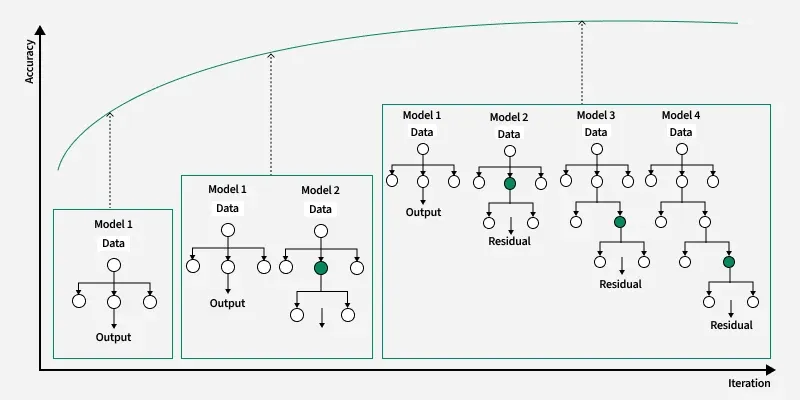
\includegraphics[width=0.85\textwidth]{lightgbm_tree_growth}
    \caption{Metode Light Gradient Boosting Machine}
    \label{fig:lightgbm_tree_growth}
\end{figure}

Gambar \ref{fig:lightgbm_tree_growth} menunjukkan mekanisme pertumbuhan pohon keputusan pada metode Light Gradient Boosting Machine (LightGBM), yaitu menggunakan pendekatan leaf-wise tree growth. Pada metode ini, proses pengembangan pohon dilakukan dengan memilih cabang (leaf) yang memiliki nilai kesalahan (loss) terbesar untuk diperluas terlebih dahulu. Artinya, model akan memprioritaskan bagian pohon yang paling membutuhkan perbaikan sehingga proses pengurangan error dapat berlangsung lebih cepat dan efektif.

Berbeda dengan metode level-wise yang mengembangkan seluruh node pada satu tingkat secara bersamaan, pendekatan leaf-wise hanya memperluas satu cabang yang paling optimal pada setiap iterasi. Strategi ini membuat struktur pohon dapat tumbuh lebih dalam pada bagian tertentu yang dianggap penting oleh model. Akibatnya, LightGBM mampu menangkap pola hubungan antar variabel yang lebih kompleks serta meningkatkan akurasi prediksi.

Pendekatan ini menjadi salah satu alasan mengapa LightGBM memiliki performa yang lebih cepat dan efisien dibandingkan metode boosting konvensional. Dengan fokus pada pengurangan error terbesar di setiap tahap, model dapat belajar dari data secara lebih terarah dan menghasilkan prediksi yang lebih optimal. Untuk memahami bagaimana LightGBM bekerja dalam proses pembelajaran model, terdapat beberapa rumus utama yang digunakan untuk mengoptimalkan fungsi objektif dan menentukan pemisahan (split) terbaik pada setiap node pohon keputusan. Rumus-rumus ini berperan dalam mengukur tingkat kesalahan model sekaligus mengontrol kompleksitas pohon agar tidak terjadi overfitting. Berikut adalah rumus inti yang digunakan dalam LightGBM:

\begin{enumerate}
    \item Fungsi Objektif (Objective Function)
    
    Fungsi objektif pada LightGBM dirumuskan sebagai berikut:
    \begin{equation}
        L = \sum_{i=1}^{n} l(y_i, \hat{y}_i) + \Omega(f)
    \end{equation}
    
    Keterangan:
    
    $l(y_i, \hat{y}_i)$ = fungsi loss (misalnya logloss untuk klasifikasi)
    
    $\Omega(f)$ = fungsi regularisasi untuk mengontrol kompleksitas model
    
    Fungsi regularisasi dirumuskan sebagai:
    \begin{equation}
        \Omega(f) = \gamma T + \frac{1}{2} \lambda \sum_{j=1}^{T} w_j^2
    \end{equation}
    
    Keterangan:
    
    $T$ = jumlah daun (leaf) pada pohon
    
    $w_j$ = nilai output pada daun ke-j
    
    $\gamma$ = parameter penalty terhadap jumlah daun
    
    $\lambda$ = parameter regularisasi L2
    
    Fungsi objektif ini bertujuan untuk meminimalkan kesalahan prediksi sekaligus menjaga agar model tidak terlalu kompleks. Regularisasi membantu mencegah overfitting dengan memberikan penalti pada jumlah daun dan besarnya bobot setiap daun.
    
    \item Rumus Gain (Pemilihan Split Terbaik)
    
    Untuk menentukan pemisahan node terbaik, LightGBM menggunakan perhitungan nilai gain sebagai berikut:
    \begin{equation}
        Gain = \frac{1}{2} \left[ \frac{G_L^2}{H_L + \lambda} + \frac{G_R^2}{H_R + \lambda} - \frac{(G_L + G_R)^2}{H_L + H_R + \lambda} \right] - \gamma
    \end{equation}
    
    Keterangan:
    
    $G_L, G_R$ = jumlah gradient pada sisi kiri dan kanan
    
    $H_L, H_R$ = jumlah hessia (gradien kedua) pada sisi kiri dan kanan
    
    $\lambda$ = parameter regularisasi L2
    
    $\gamma$ = penalti terhadap jumlah daun
    
    Rumus gain ini digunakan untuk mengevaluasi apakah suatu pemisahan node memberikan peningkatan kualitas model atau tidak. Semakin besar nilai gain, maka semakin baik pemisahan tersebut dalam mengurangi error.
\end{enumerate}

Melalui kombinasi fungsi objektif dan perhitungan gain tersebut, LightGBM mampu membangun struktur pohon keputusan secara efisien dan terarah. Fungsi objektif memastikan model tetap optimal dan tidak overfitting, sedangkan rumus gain membantu memilih pemisahan node terbaik pada setiap tahap pembentukan pohon. Dengan mekanisme ini, LightGBM dapat menghasilkan model klasifikasi yang cepat, stabil, dan memiliki performa tinggi pada berbagai jenis dataset.


%%=============================================================
%%=============================================================
%%=============================================================
%%=============================================================
%% BAB III - METODOLOGI PENELITIAN
%%=============================================================
\chapter[METODOLOGI PENELITIAN]{\\ METODOLOGI PENELITIAN}

\section{Data dan Pengumpulan data}
Tahap pengumpulan data merupakan langkah awal yang penting dalam penelitian untuk memastikan ketersediaan data yang relevan dalam proses klasifikasi kelayakan penerima subsidi listrik rumah tangga. Data yang digunakan dalam penelitian ini merupakan kombinasi antara data sekunder dan data sintetis. Data sekunder diperoleh dari Dinas Sosial dan berjumlah 1.000 data rumah tangga yang memuat informasi mengenai kondisi sosial ekonomi masyarakat. Sementara itu, data sintetis digunakan untuk melengkapi atribut teknis kelistrikan yang tidak tersedia pada data Dinas Sosial.

Data sintetis merupakan data buatan yang dibangkitkan secara sistematis sehingga memiliki karakteristik yang menyerupai data nyata. Dalam penelitian ini, pembangkitan data sintetis dilakukan menggunakan pendekatan \textit{rule-based synthetic data generation}, yaitu menghasilkan data berdasarkan aturan yang mengacu pada karakteristik sosial ekonomi yang tersedia pada data Dinas Sosial serta ketentuan penerima subsidi listrik yang diatur dalam regulasi Kementerian Energi dan Sumber Daya Mineral (ESDM). Atribut yang dibangkitkan meliputi daya listrik terpasang (VA), golongan tarif, dan penggunaan listrik per bulan (kWh). Proses ini dilakukan agar dataset memiliki informasi yang lebih lengkap sehingga dapat digunakan dalam proses pelatihan model klasifikasi.

Data yang digunakan dalam penelitian ini terdiri atas beberapa komponen sebagai berikut:
\begin{enumerate}
    \item \textbf{Data Sosial Ekonomi} \\
    Data sosial ekonomi merupakan data sekunder yang diperoleh dari Dinas Sosial. Variabel yang digunakan meliputi:
    \begin{enumerate}
        \item Penghasilan keluarga.
        \item Jumlah anggota keluarga.
        \item Pekerjaan kepala keluarga.
        \item Status kepemilikan rumah.
        \item Luas bangunan.
        \item Status penerima bantuan sosial (PKH/BPNT).
    \end{enumerate}
    \item \textbf{Data Karakteristik Kelistrikan} \\
    Data karakteristik kelistrikan merupakan data sintetis yang dibangkitkan berdasarkan karakteristik pelanggan rumah tangga dan mengacu pada regulasi Kementerian ESDM mengenai penerima subsidi listrik. Variabel yang digunakan meliputi:
    \begin{enumerate}
        \item Daya listrik terpasang (VA).
        \item Golongan tarif listrik.
        \item Penggunaan listrik per bulan (kWh).
    \end{enumerate}
    \item \textbf{Data Label Klasifikasi} \\
    Data label digunakan sebagai variabel target (\textit{output}) dalam proses pembelajaran algoritma Light Gradient Boosting Machine (LightGBM). Label menunjukkan status kelayakan pelanggan dalam menerima subsidi listrik yang ditentukan berdasarkan kombinasi karakteristik sosial ekonomi dan karakteristik kelistrikan sesuai kriteria yang mengacu pada regulasi Kementerian ESDM. Label klasifikasi terdiri atas:
    \begin{enumerate}
        \item Layak menerima subsidi.
        \item Tidak layak menerima subsidi.
    \end{enumerate}
\end{enumerate}
Seluruh variabel tersebut digunakan sebagai fitur masukan dalam proses pelatihan dan pengujian model menggunakan algoritma Light Gradient Boosting Machine (LightGBM). Dengan mengombinasikan data sosial ekonomi dari Dinas Sosial dan data kelistrikan sintetis yang dibangkitkan berdasarkan regulasi Kementerian ESDM, diharapkan model mampu mempelajari pola hubungan antara karakteristik pelanggan dengan status kelayakan penerima subsidi listrik secara objektif dan menghasilkan performa klasifikasi yang baik.

\subsection{Sumber Data}
Sumber data penelitian ini terbagi menjadi dua jenis:
\begin{enumerate}
    \item \textbf{Data Sekunder} \\
    Data sekunder merupakan data yang diperoleh dari sumber yang telah tersedia tanpa melakukan pengumpulan data secara langsung dari objek penelitian. Pada penelitian ini, data sekunder terdiri atas dua jenis, yaitu:
    \begin{enumerate}
        \item Data sosial ekonomi masyarakat yang diperoleh dari Dinas Sosial, meliputi informasi seperti penghasilan keluarga, jumlah anggota keluarga, pekerjaan kepala keluarga, status kepemilikan rumah, luas bangunan, dan status penerima bantuan sosial (PKH/BPNT).
        \item Literatur pendukung yang diperoleh dari jurnal ilmiah, buku, penelitian terdahulu, serta regulasi Kementerian Energi dan Sumber Daya Mineral (ESDM) yang berkaitan dengan subsidi listrik dan penerapan algoritma Light Gradient Boosting Machine (LightGBM).
    \end{enumerate}
    \item \textbf{Data Sintetis} \\
    Data sintetis merupakan data buatan yang dibangkitkan untuk melengkapi atribut yang tidak tersedia pada data sekunder. Dalam penelitian ini, data sintetis dibentuk menggunakan pendekatan \textit{rule-based synthetic data generation}, yaitu pembangkitan data berdasarkan aturan yang mengacu pada karakteristik data sosial ekonomi dari Dinas Sosial dan regulasi Kementerian ESDM mengenai penerima subsidi listrik. Atribut yang dibangkitkan meliputi daya listrik terpasang (VA), golongan tarif, penggunaan listrik per bulan (kWh), serta label kelayakan penerima subsidi listrik (Layak/Tidak Layak). Data sintetis tersebut digunakan sebagai dataset pelatihan dan pengujian model klasifikasi menggunakan algoritma LightGBM.
\end{enumerate}

\section{Analisis Kebutuhan Sistem}
Analisis kebutuhan sistem dilakukan untuk mengidentifikasi kebutuhan yang diperlukan dalam pembangunan sistem klasifikasi kelayakan penerima subsidi listrik pelanggan PLN Aceh menggunakan metode Light Gradient Boosting Machine (LightGBM). Tahap ini bertujuan untuk memastikan sistem yang dikembangkan mampu mendukung seluruh proses penelitian mulai dari pengolahan data, pelatihan model, hingga penyajian hasil klasifikasi secara efektif dan terstruktur.

Kebutuhan sistem pada penelitian ini dibagi menjadi dua kategori utama, yaitu kebutuhan fungsional dan kebutuhan non-fungsional. Kebutuhan fungsional menjelaskan layanan sistem yang harus tersedia, sedangkan kebutuhan non-fungsional berkaitan dengan spesifikasi perangkat keras dan perangkat lunak yang digunakan dalam proses pengembangan dan pengujian sistem.

\subsection{Kebutuhan Fungsional}
Kebutuhan fungsional menggambarkan kemampuan atau layanan utama yang harus dimiliki sistem agar dapat menjalankan proses klasifikasi kelayakan penerima subsidi listrik secara optimal. Sistem yang dikembangkan berfungsi sebagai alat analisis data berbasis machine learning yang digunakan oleh peneliti dalam melakukan pengolahan dan evaluasi model. Kebutuhan fungsional ini dirancang agar seluruh tahapan pengolahan data hingga penyajian hasil analisis dapat berjalan secara sistematis dan terintegrasi. Berikut merupakan kebutuhan fungsional sistem yang meliputi:
\begin{enumerate}
    \item \textbf{Import Dataset} \\
    Sistem mampu menerima dan membaca dataset pelanggan listrik dalam format file digital seperti CSV atau Microsoft Excel. Dataset yang diimpor berisi data administratif pelanggan serta data konsumsi listrik yang akan digunakan sebagai bahan utama dalam proses analisis dan pelatihan model klasifikasi. Sistem juga harus mampu memastikan bahwa struktur data sesuai dengan format yang dibutuhkan sehingga data dapat diproses pada tahap selanjutnya tanpa kesalahan pembacaan.
    \item \textbf{Preprocessing Data} \\
    Sistem mampu melakukan proses persiapan data sebelum digunakan dalam pelatihan model machine learning. Tahap preprocessing bertujuan untuk meningkatkan kualitas data agar menghasilkan model yang lebih akurat dan stabil. Proses preprocessing meliputi:
    \begin{enumerate}
        \item Pembersihan data (\textit{data cleaning}) untuk menghapus data duplikat atau data tidak valid.
        \item Penanganan data kosong (\textit{missing value handling}).
        \item Transformasi data agar sesuai dengan format analisis.
        \item Encoding variabel kategorikal menjadi bentuk numerik yang dapat diproses oleh algoritma.
        \item Pembagian dataset menjadi data training dan data testing sebagai dasar pelatihan dan pengujian model.
    \end{enumerate}
    \item \textbf{Pelatihan Model (Training Model)} \\
    Sistem mampu melakukan proses pelatihan model klasifikasi menggunakan algoritma Light Gradient Boosting Machine (LightGBM). Pada tahap ini, sistem mempelajari pola hubungan antara karakteristik pelanggan listrik dengan status kelayakan subsidi berdasarkan data training yang telah diproses sebelumnya, sehingga model dapat digunakan untuk melakukan prediksi terhadap data baru.
    \item \textbf{Prediksi Klasifikasi} \\
    Sistem mampu melakukan prediksi status kelayakan subsidi listrik pelanggan secara otomatis menggunakan model yang telah dilatih. Hasil prediksi berupa kategori pelanggan yang diklasifikasikan sebagai layak atau tidak layak menerima subsidi listrik berdasarkan karakteristik data pelanggan.
    \item \textbf{Evaluasi Model} \\
    Sistem mampu melakukan evaluasi performa model klasifikasi untuk mengetahui tingkat akurasi dan kualitas prediksi yang dihasilkan. Evaluasi dilakukan menggunakan beberapa metrik pengukuran performa, yaitu:
    \begin{enumerate}
        \item Accuracy untuk mengukur tingkat ketepatan prediksi secara keseluruhan.
        \item Precision untuk mengukur ketepatan prediksi pada kelas tertentu.
        \item Recall untuk mengukur kemampuan model dalam menemukan data yang relevan.
        \item F1-Score sebagai kombinasi nilai precision dan recall.
        \item Confusion Matrix untuk menampilkan perbandingan antara hasil prediksi dan data aktual secara detail.
    \end{enumerate}
    \item \textbf{Menampilkan Hasil Analisis} \\
    Sistem mampu menampilkan hasil klasifikasi pelanggan beserta nilai evaluasi model dalam bentuk tabel, grafik, atau laporan analisis sehingga memudahkan pengguna dalam memahami hasil pengolahan data dan performa model yang telah dibangun.
    \item \textbf{Penyimpanan Hasil} \\
    Sistem mampu menyimpan dataset hasil pengolahan, model yang telah dilatih, serta hasil prediksi klasifikasi ke dalam media penyimpanan atau database.
\end{enumerate}

\subsection{Kebutuhan Non-Fungsional}
Kebutuhan non-fungsional merupakan kebutuhan pendukung yang berkaitan dengan spesifikasi teknis sistem agar proses pengembangan dan pengujian model dapat berjalan dengan baik. Kebutuhan ini mencakup perangkat keras dan perangkat lunak yang digunakan dalam penelitian.

\begin{enumerate}
    \item \textbf{Kebutuhan Perangkat Keras (Hardware)} \\
    Perangkat keras digunakan untuk menjalankan proses pengolahan data dan pelatihan model machine learning yang membutuhkan kemampuan komputasi tertentu.
    \begin{table}[H]
    \setstretch{1.2}
    \centering
    \caption{Kebutuhan Perangkat Keras (Hardware)}
    \label{tab:hardware_req}
    \begin{tabularx}{\textwidth}{|c|p{2.8cm}|p{5cm}|X|}
    \hline
    \textbf{No} & \textbf{Nama Perangkat} & \textbf{Spesifikasi} & \textbf{Keterangan} \\ \hline
    1 & Laptop / PC & Processor Intel Core i5 / setara & Perangkat utama pengembangan sistem \\ \hline
    2 & RAM & 8 GB & Mendukung proses training model \\ \hline
    3 & Penyimpanan & 256 GB SSD & Penyimpanan dataset dan hasil model \\ \hline
    \end{tabularx}
    \end{table}

    \item \textbf{Kebutuhan Perangkat Lunak (Software)} \\
    Perangkat lunak digunakan sebagai lingkungan utama dalam proses pengembangan sistem, pengolahan data, serta implementasi algoritma Light Gradient Boosting Machine (LightGBM) pada penelitian ini.
    \begin{table}[H]
    \setstretch{1.2}
    \centering
    \caption{Kebutuhan Perangkat Lunak (Software)}
    \label{tab:software_req}
    \begin{tabularx}{\textwidth}{|c|p{3.5cm}|p{5.5cm}|X|}
    \hline
    \textbf{No} & \textbf{Software} & \textbf{Spesifikasi} & \textbf{Fungsi} \\ \hline
    1 & Sistem Operasi & Windows / Linux & Platform menjalankan sistem \\ \hline
    2 & Python & Bahasa pemrograman utama & - \\ \hline
    3 & Jupyter Notebook / Colab & Lingkungan eksperimen machine learning & - \\ \hline
    4 & Library Pandas \& NumPy & Pengolahan dan manipulasi data & - \\ \hline
    5 & Scikit-Learn & Preprocessing dan evaluasi model & - \\ \hline
    6 & LightGBM Library & Implementasi algoritma LightGBM & - \\ \hline
    7 & Visual Studio Code & Editor kode program & - \\ \hline
    8 & Microsoft Excel & Pengolahan awal dataset & - \\ \hline
    9 & Draw.io & Perancangan diagram sistem & - \\ \hline
    \end{tabularx}
    \end{table}
\end{enumerate}

\section{Rancangan Sistem}
Rancangan sistem merupakan tahap perencanaan yang dilakukan untuk menggambarkan alur kerja sistem klasifikasi kelayakan penerima subsidi listrik menggunakan metode Light Gradient Boosting Machine (LightGBM). Perancangan ini bertujuan untuk memberikan gambaran mengenai proses pengolahan data, interaksi pengguna dengan sistem, serta tahapan analisis yang dilakukan mulai dari input data hingga menghasilkan output klasifikasi. Rancangan sistem divisualisasikan menggunakan diagram UML agar alur sistem dapat dipahami secara jelas sebelum tahap implementasi dilakukan.

\subsection{Arsitektur Sistem}
Arsitektur sistem menggambarkan struktur dan alur kerja utama sistem dalam mengolah data pelanggan listrik hingga menghasilkan hasil klasifikasi kelayakan subsidi. Sistem dirancang dalam beberapa tahapan, yaitu proses input data, preprocessing data, pelatihan model LightGBM, penyimpanan data, serta penyajian output hasil analisis. Arsitektur ini menunjukkan hubungan antar komponen sistem yang saling terintegrasi dalam proses klasifikasi.

\begin{figure}[H]
    \centering
    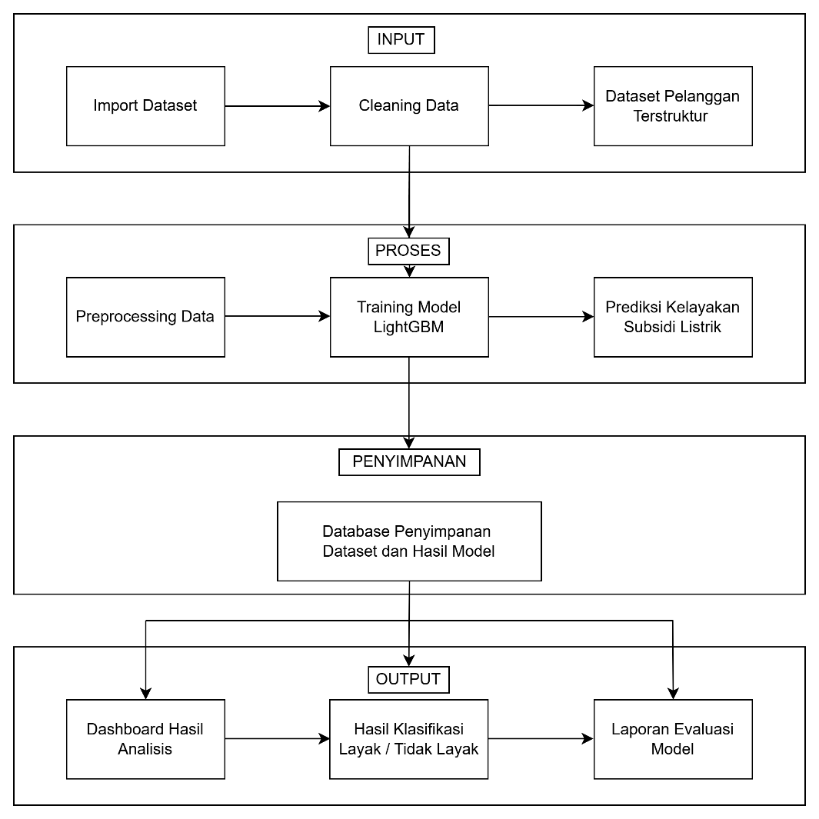
\includegraphics[width=0.85\textwidth]{arsitektur_sistem}
    \caption{Arsitektur Sistem}
    \label{fig:arsitektur_sistem}
\end{figure}

Gambar \ref{fig:arsitektur_sistem} menunjukkan arsitektur sistem klasifikasi kelayakan penerima subsidi listrik yang terdiri dari empat tahapan utama. Pada tahap input, sistem menerima dataset pelanggan listrik yang kemudian melalui proses cleaning data untuk menghasilkan dataset yang terstruktur. Tahap proses meliputi preprocessing data serta pelatihan model menggunakan algoritma Light Gradient Boosting Machine (LightGBM) untuk menghasilkan prediksi kelayakan subsidi listrik. Hasil pengolahan data dan model selanjutnya disimpan pada database sebagai tahap penyimpanan. Pada tahap output, sistem menampilkan hasil analisis berupa dashboard, hasil klasifikasi pelanggan layak atau tidak layak menerima subsidi, serta laporan evaluasi performa model.

\subsection{Use Case Diagram}
Use Case Diagram digunakan untuk menggambarkan fungsi utama sistem serta interaksi antara pengguna dengan sistem klasifikasi kelayakan penerima subsidi listrik yang dikembangkan. Diagram ini memberikan gambaran umum mengenai layanan yang disediakan sistem serta aktivitas yang dapat dilakukan oleh pengguna selama proses pengolahan data hingga memperoleh hasil klasifikasi.

\begin{figure}[H]
    \centering
    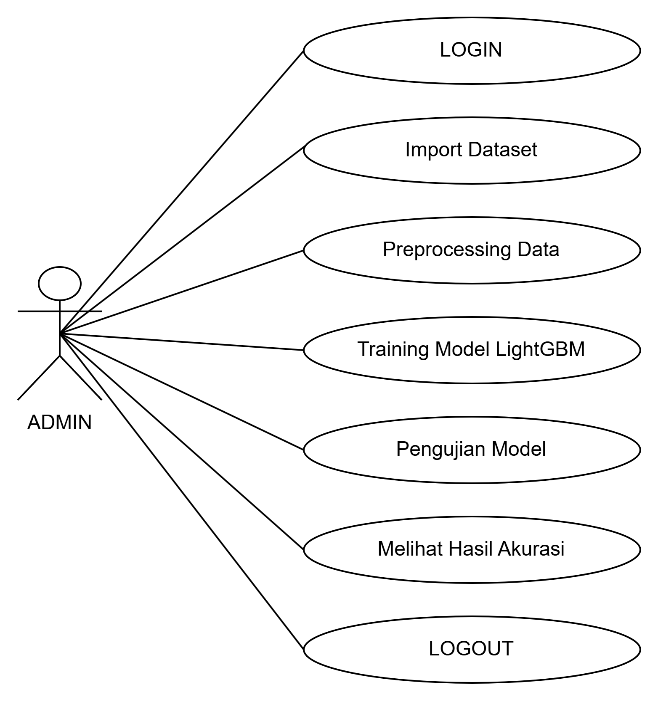
\includegraphics[width=0.85\textwidth]{use_case_diagram}
    \caption{Use Case Diagram}
    \label{fig:use_case_diagram}
\end{figure}

Use Case Diagram pada Gambar \ref{fig:use_case_diagram} menggambarkan interaksi antara pengguna dengan sistem klasifikasi kelayakan penerima subsidi listrik. Pengguna dapat melakukan beberapa aktivitas utama, yaitu login ke dalam sistem, mengimpor dataset pelanggan listrik, melakukan preprocessing data, menjalankan proses pelatihan model menggunakan algoritma LightGBM, melakukan pengujian model, serta melihat hasil akurasi klasifikasi yang dihasilkan. Setelah seluruh proses selesai, pengguna dapat keluar dari sistem melalui fitur logout. Diagram ini menunjukkan fungsi-fungsi utama sistem yang mendukung proses analisis data secara terstruktur dan sistematis.

\subsection{Activity Diagram}
Activity Diagram adalah diagram yang memodelkan aliran aktivitas pada sistem. Adapun Activity Diagram pada sistem adalah sebagai berikut:

\begin{enumerate}
    \item \textbf{Activity Diagram Login} \\
    Activity Diagram Login adalah gambaran proses login ke dalam sistem dapat dilihat pada Gambar \ref{fig:act_login} berikut.
    \begin{figure}[H]
        \centering
        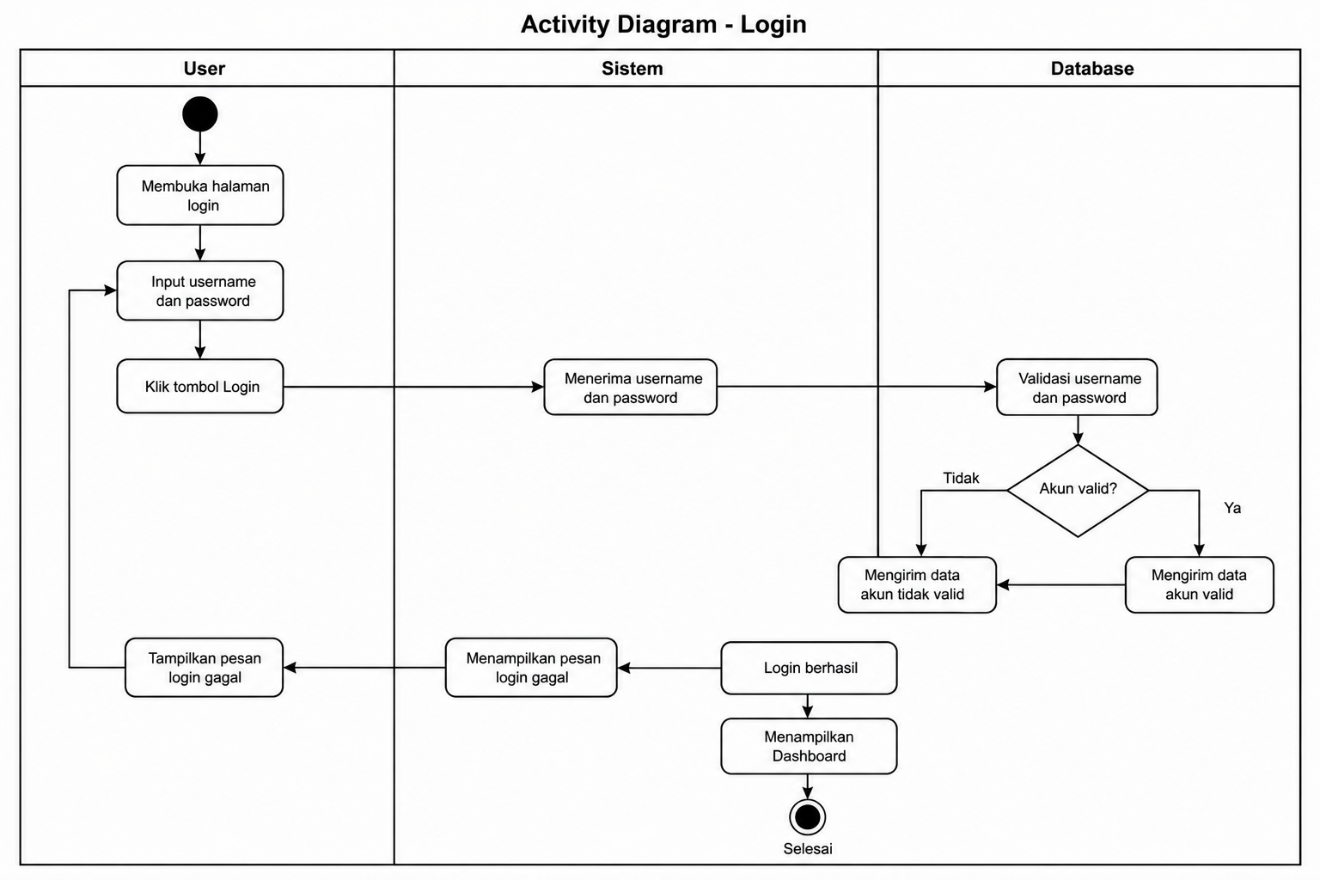
\includegraphics[width=0.7\textwidth]{act_login}
        \caption{Activity Diagram Login}
        \label{fig:act_login}
    \end{figure}
    Gambar \ref{fig:act_login} menggambarkan Activity Diagram untuk proses login. Pada tahap awal, admin memasukkan username dan password ke dalam sistem. Setelah itu, admin menekan tombol login. Sistem kemudian melakukan verifikasi terhadap username dan password yang dimasukkan dengan melakukan pencarian pada database untuk mencocokkan informasi tersebut. Selanjutnya, sistem akan melakukan pengecekan apakah informasi yang dimasukkan benar atau tidak. Jika informasi yang dimasukkan sesuai dengan data yang ada di database, maka sistem akan memberikan hak akses kepada admin dan menampilkan halaman utama sistem klasifikasi. Namun, jika tidak ditemukan informasi yang sesuai, sistem akan menampilkan halaman login gagal.

    \item \textbf{Activity Diagram Halaman Dashboard} \\
    Activity Diagram halaman Dashboard menjelaskan alur proses yang terjadi saat pengguna membuka halaman Dashboard. Sistem mengambil data dari database, mengolah informasi yang diperlukan, kemudian menampilkan ringkasan hasil klasifikasi beserta informasi pendukung kepada pengguna.
    \begin{figure}[H]
        \centering
        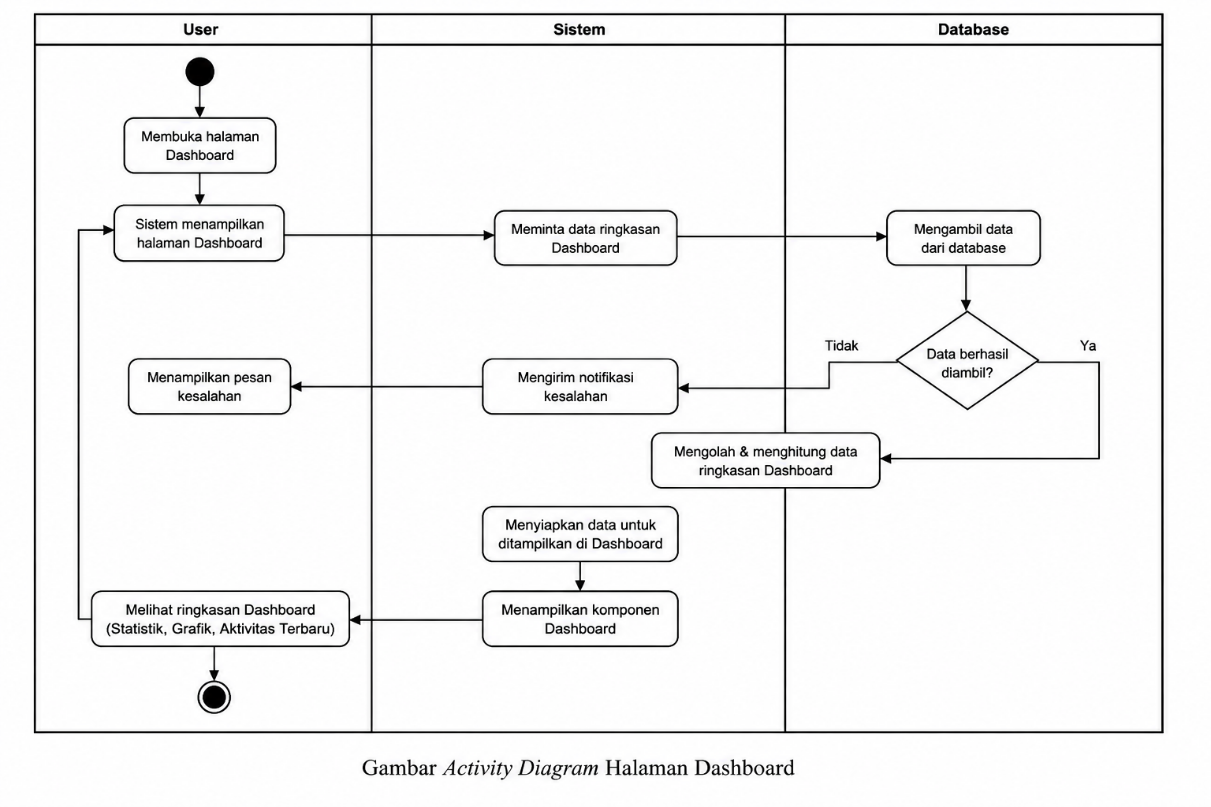
\includegraphics[width=0.75\textwidth]{act_dashboard}
        \caption{Activity Diagram Dashboard}
        \label{fig:act_dashboard}
    \end{figure}
    Pada Gambar \ref{fig:act_dashboard} di atas menampilkan activity diagram halaman Dashboard yang menggambarkan alur aktivitas ketika pengguna mengakses halaman Dashboard setelah berhasil melakukan login. Proses diawali dengan pengguna membuka halaman Dashboard, kemudian sistem mengirimkan permintaan untuk mengambil data ringkasan dari database. Selanjutnya, database mengembalikan data yang dibutuhkan kepada sistem untuk diproses. Jika proses pengambilan data berhasil, sistem mengolah data tersebut menjadi informasi berupa total pelanggan yang dianalisis, rasio kelayakan subsidi, total laporan yang tersimpan, distribusi hasil klasifikasi, serta aktivitas terbaru. Setelah seluruh data selesai diproses, sistem menampilkan seluruh komponen Dashboard sehingga pengguna dapat melihat ringkasan informasi secara lengkap. Apabila terjadi kegagalan dalam proses pengambilan data, sistem akan menampilkan pesan kesalahan kepada pengguna.

    \item \textbf{Activity Diagram Halaman Klasifikasi} \\
    Activity Diagram pada halaman Klasifikasi Baru menggambarkan alur proses klasifikasi kelayakan penerima subsidi listrik melalui dua metode, yaitu Input Manual dan Upload Batch. Diagram ini menunjukkan interaksi antara pengguna, sistem, dan database.
    \begin{figure}[H]
        \centering
        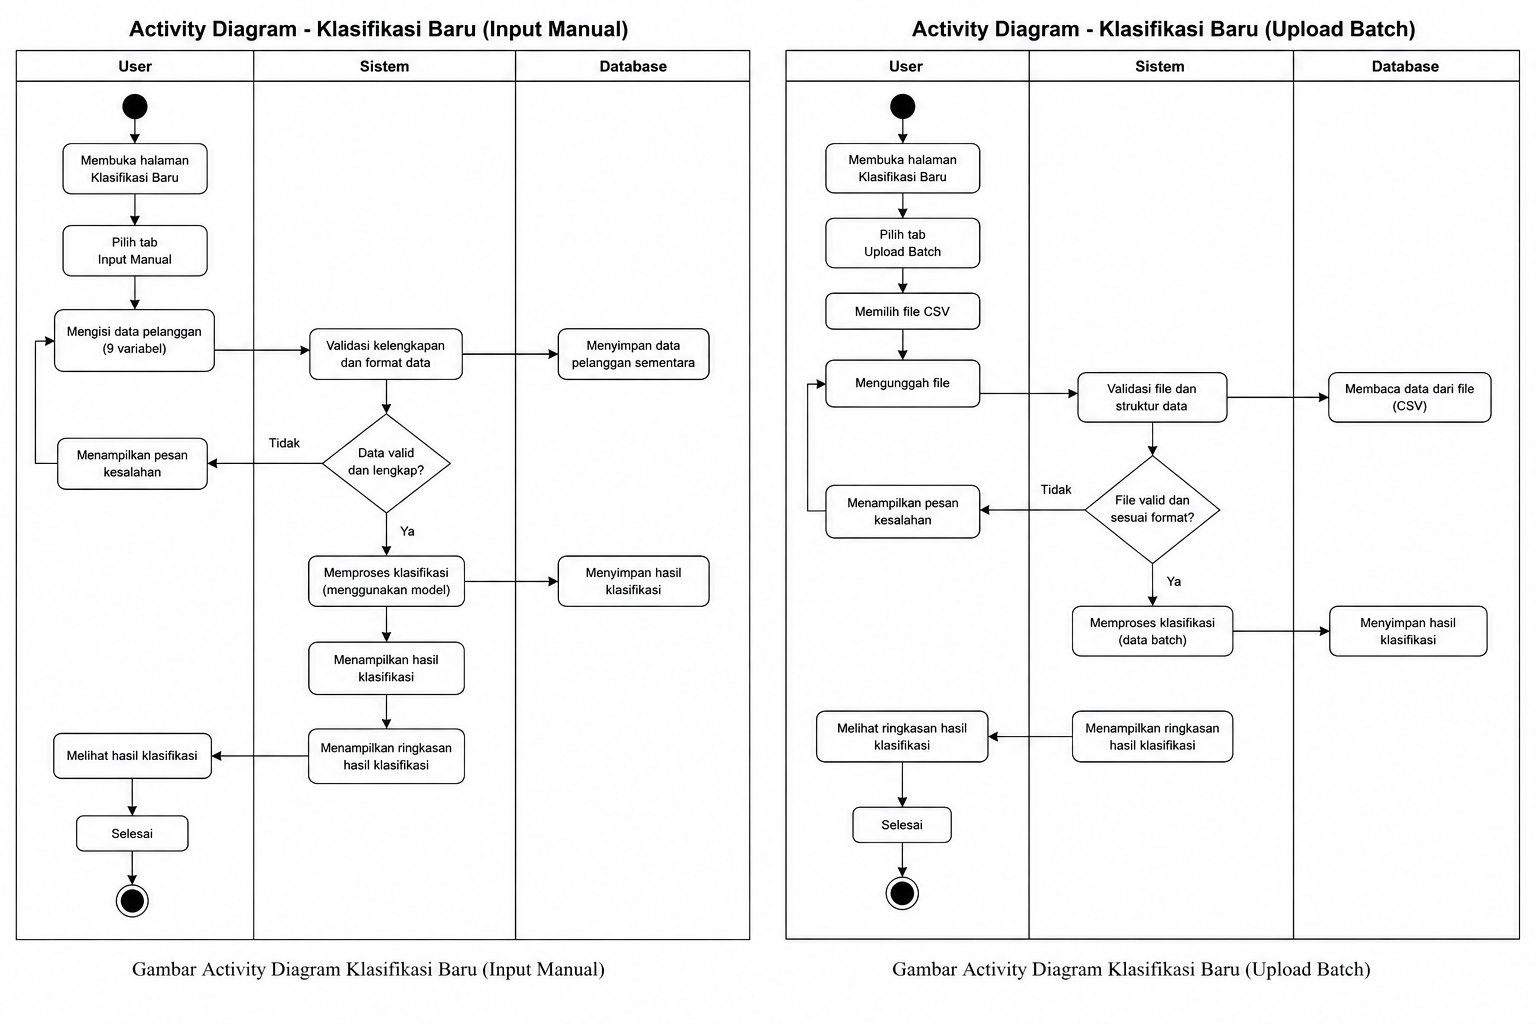
\includegraphics[width=0.75\textwidth]{act_klasifikasi_manual}
        \caption{Activity Diagram Klasifikasi Manual}
        \label{fig:act_klasifikasi_manual}
    \end{figure}
    \begin{figure}[H]
        \centering
        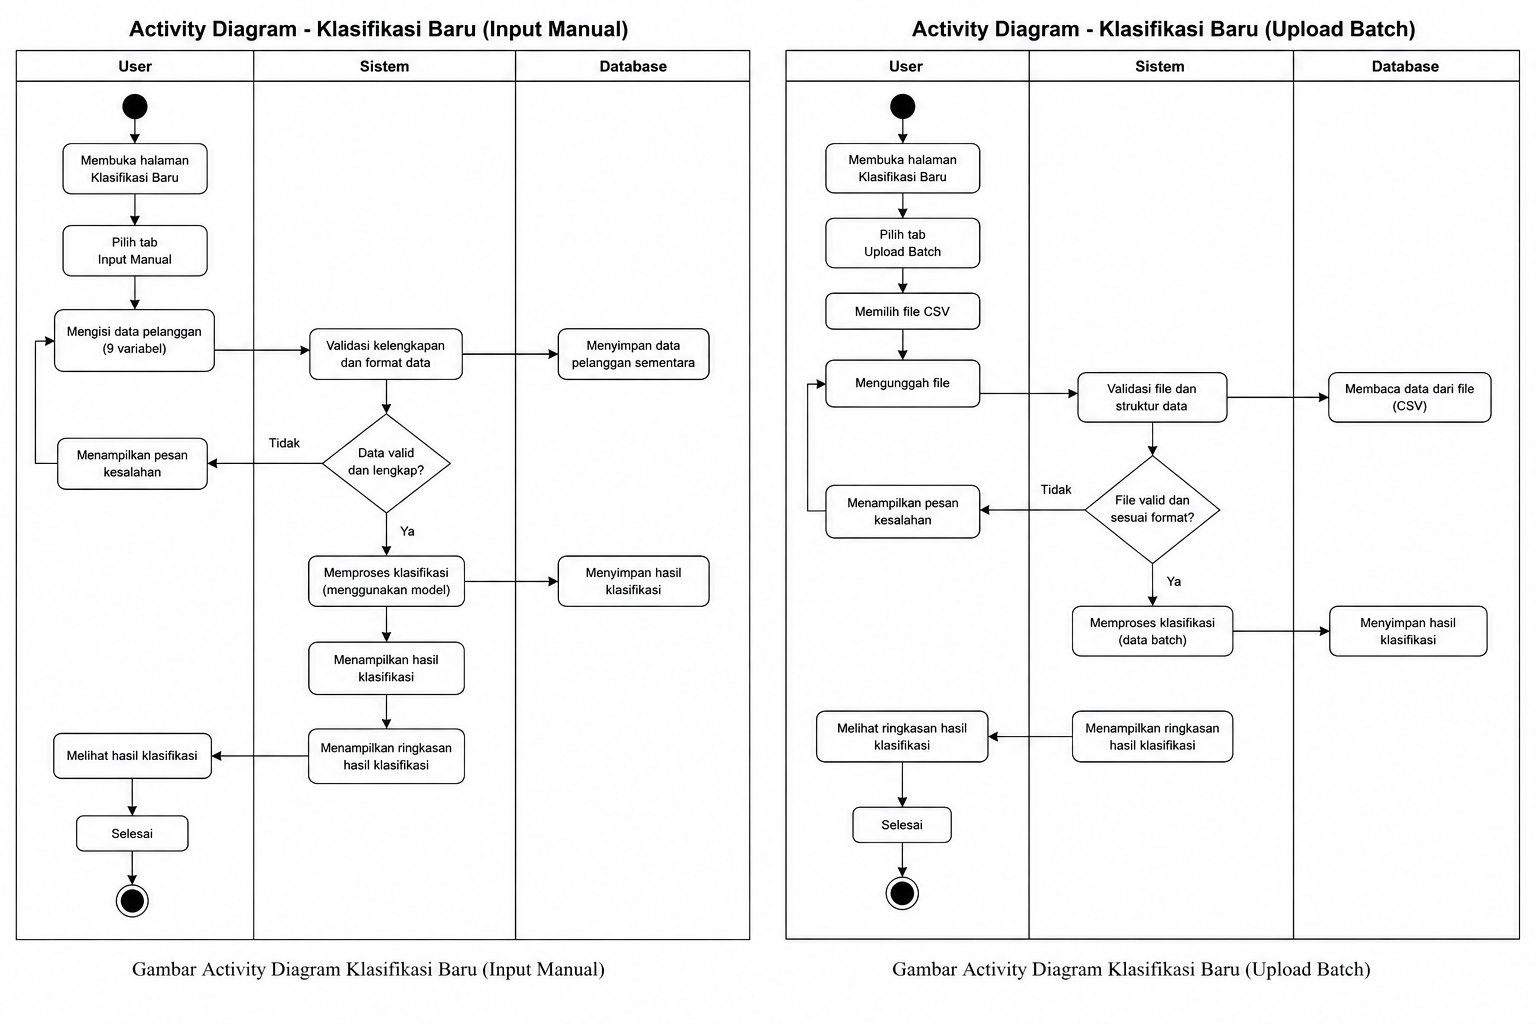
\includegraphics[width=0.75\textwidth]{act_klasifikasi_batch}
        \caption{Activity Diagram Klasifikasi Batch}
        \label{fig:act_klasifikasi_batch}
    \end{figure}
    Gambar \ref{fig:act_klasifikasi_manual} and Gambar \ref{fig:act_klasifikasi_batch} menunjukkan alur aktivitas untuk masing-masing metode input manual dan upload batch secara lengkap dari awal penginputan/upload hingga hasil prediksi kelayakan ditampilkan dan disimpan ke database.

    \item \textbf{Activity Diagram Halaman Riwayat Klasifikasi} \\
    Activity Diagram pada halaman Riwayat Klasifikasi menggambarkan alur aktivitas untuk menelusuri, memfilter, dan mengekspor laporan hasil klasifikasi kelayakan penerima subsidi listrik yang telah dilakukan sebelumnya. Alur ini dapat dilihat pada Gambar \ref{fig:act_riwayat_klasifikasi} berikut.
    \begin{figure}[H]
        \centering
        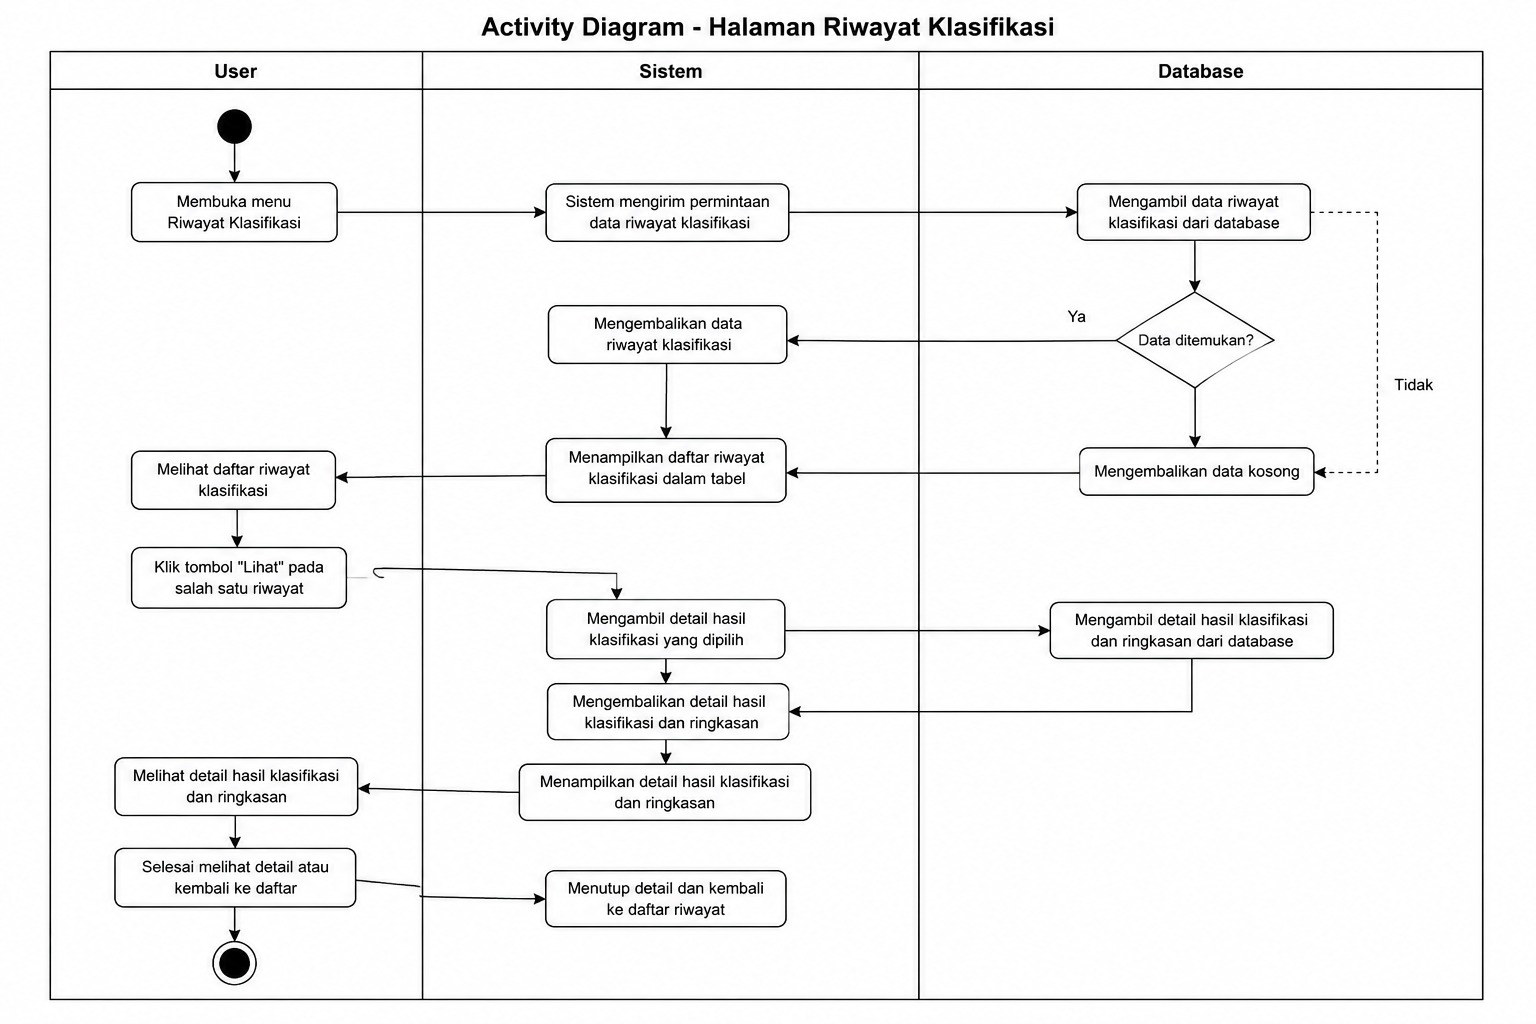
\includegraphics[width=0.75\textwidth]{act_riwayat_klasifikasi}
        \caption{Activity Diagram Riwayat Klasifikasi}
        \label{fig:act_riwayat_klasifikasi}
    \end{figure}
    Pada Gambar \ref{fig:act_riwayat_klasifikasi} di atas menunjukkan aliran proses di mana admin membuka halaman laporan, kemudian sistem memanggil database untuk menyajikan daftar data riwayat kelayakan. Admin dapat melakukan penyaringan (filtering) berdasarkan kategori tertentu atau mengekspor laporan tersebut menjadi dokumen PDF/Excel yang kemudian diunduh secara lokal.

    \item \textbf{Activity Diagram Halaman Laporan} \\
    Activity Diagram pada halaman Laporan menggambarkan alur proses penyajian ringkasan statistik dan grafik distribusi hasil klasifikasi penerima subsidi listrik dalam bentuk laporan berkala. Alur ini dapat dilihat pada Gambar \ref{fig:act_halaman_laporan} berikut.
    \begin{figure}[H]
        \centering
        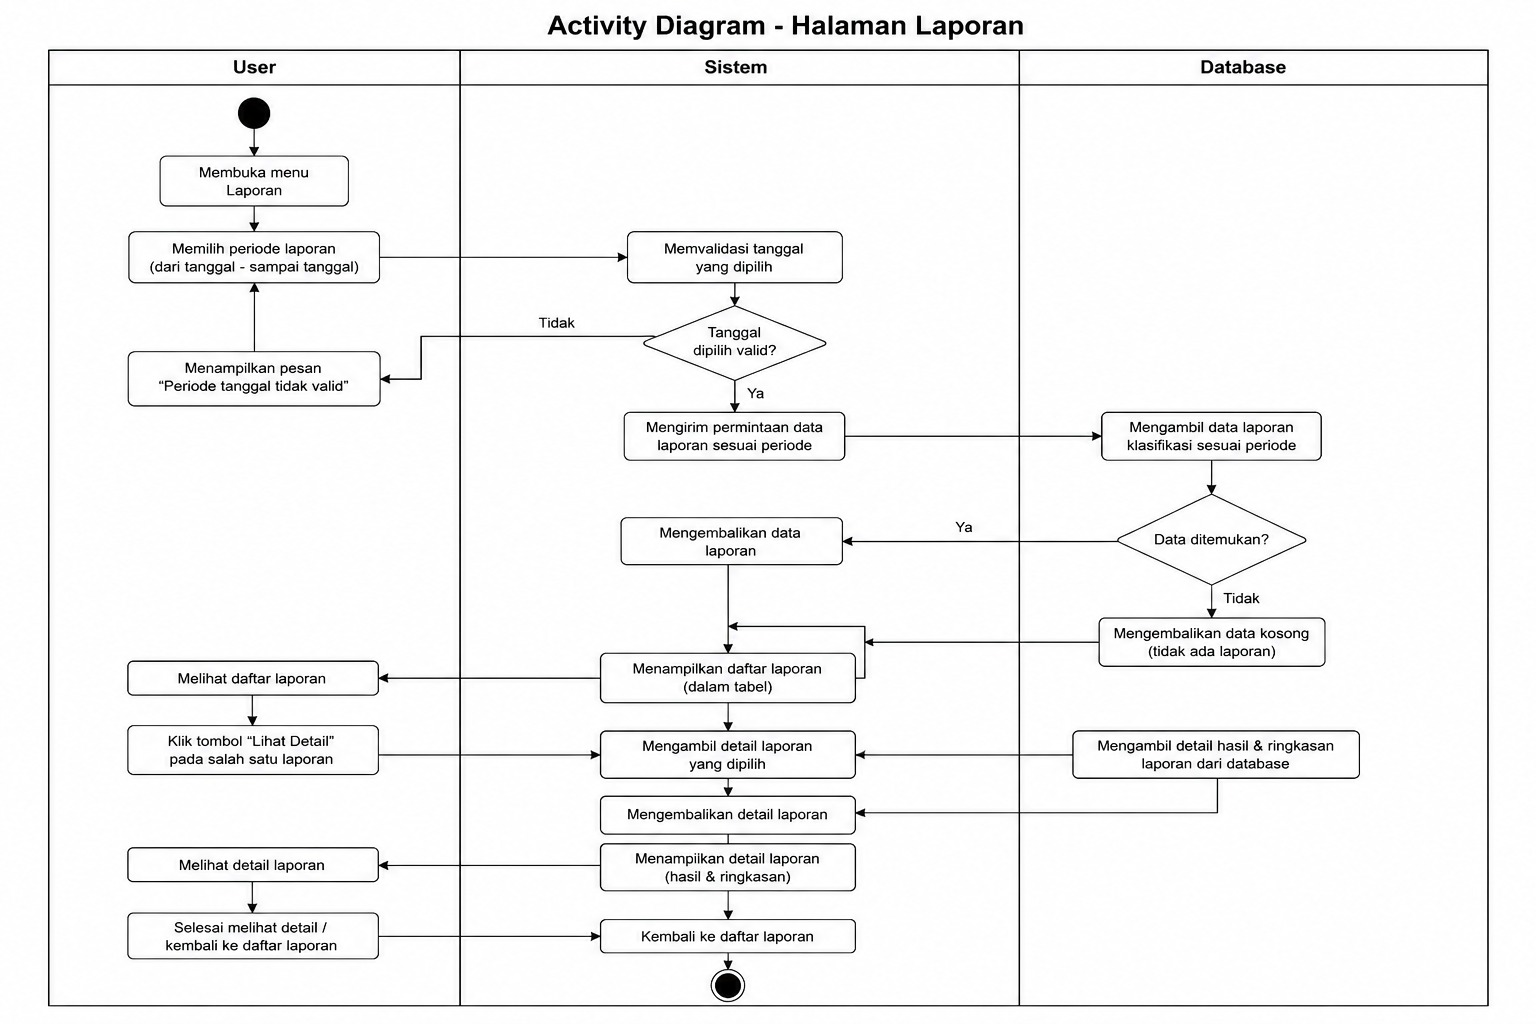
\includegraphics[width=0.75\textwidth]{act_halaman_laporan}
        \caption{Activity Diagram Halaman Laporan}
        \label{fig:act_halaman_laporan}
    \end{figure}
    Pada Gambar \ref{fig:act_halaman_laporan} di atas menunjukkan alur aktivitas ketika admin membuka menu laporan. Sistem akan memproses dan menampilkan rekapitulasi data kelayakan subsidi listrik, visualisasi grafik tren bulanan, serta menyediakan opsi ekspor laporan cetak bagi admin.

    \item \textbf{Activity Diagram Halaman Pengaturan} \\
    Activity Diagram pada halaman Pengaturan Model menggambarkan alur kerja verifikasi status model aktif, konfigurasi parameter LightGBM, serta proses pelatihan ulang (\textit{retraining}) model klasifikasi secara dinamis. Alur ini dapat dilihat pada Gambar \ref{fig:act_halaman_pengaturan} berikut.
    \begin{figure}[H]
        \centering
        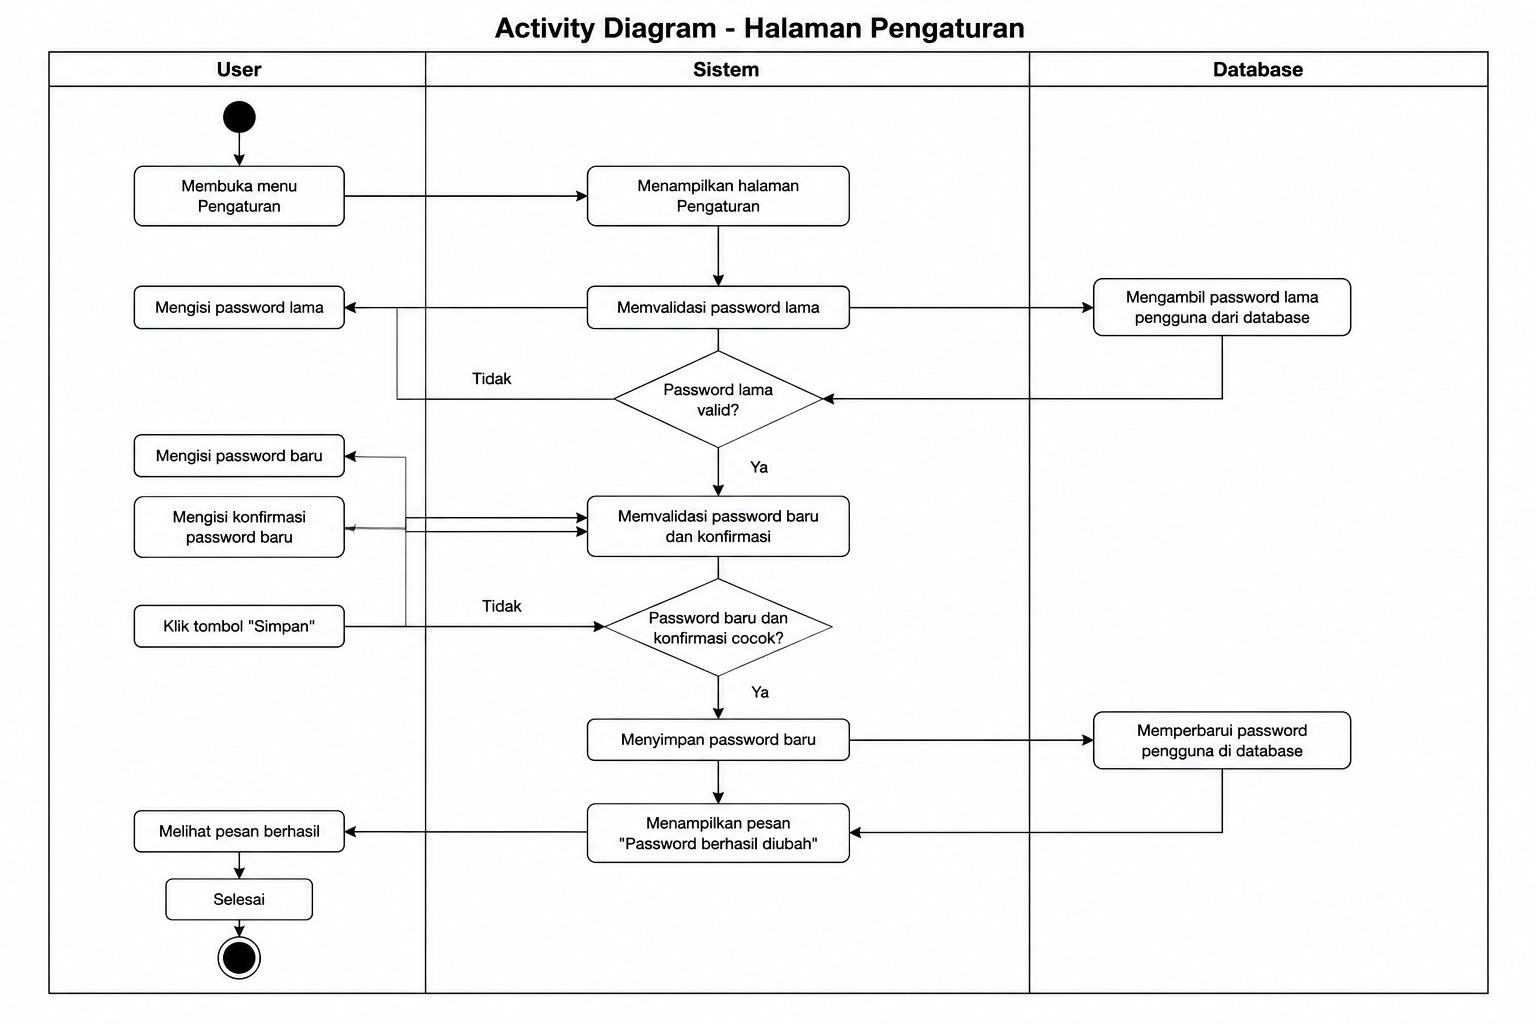
\includegraphics[width=0.75\textwidth]{act_halaman_pengaturan}
        \caption{Activity Diagram Halaman Pengaturan Model}
        \label{fig:act_halaman_pengaturan}
    \end{figure}
    Pada Gambar \ref{fig:act_halaman_pengaturan} di atas menunjukkan proses ketika admin masuk ke menu pengaturan model. Sistem menampilkan konfigurasi parameter dan performa model saat ini. Admin dapat menginisiasi proses training model baru dengan data tambahan, di mana sistem mengirimkan instruksi ke server API Flask untuk melatih kembali model LightGBM secara asinkron.
\end{enumerate}

\section{Metode dan Variabel Penelitian}
Metode dan variabel penelitian digunakan sebagai dasar dalam proses pembangunan model klasifikasi kelayakan penerima subsidi listrik pelanggan PLN Aceh. Pada penelitian ini digunakan pendekatan machine learning berbasis supervised learning dengan algoritma Light Gradient Boosting Machine (LightGBM). Metode tersebut dipilih karena memiliki kemampuan klasifikasi yang baik serta efisien dalam menangani data berukuran besar dan hubungan nonlinier antar variabel. Proses penelitian dilakukan dengan memanfaatkan data pelanggan listrik sebagai variabel input untuk menghasilkan prediksi status kelayakan subsidi listrik sebagai variabel output.

\section{Teknik Pengujian}
Teknik pengujian sistem pada penelitian ini dilakukan untuk memastikan bahwa sistem klasifikasi kelayakan penerima subsidi listrik dapat berjalan sesuai dengan fungsi yang telah dirancang serta mampu menghasilkan prediksi yang akurat. Pengujian dilakukan terhadap fungsi sistem maupun performa model klasifikasi yang dibangun menggunakan algoritma Light Gradient Boosting Machine (LightGBM). Pengujian dalam penelitian ini menggunakan dua pendekatan utama, yaitu pengujian fungsional sistem menggunakan metode Blackbox Testing dan pengujian performa model menggunakan metrik evaluasi klasifikasi.

\subsection{Pengujian Black Box}
Pengujian Blackbox merupakan metode pengujian perangkat lunak yang berfokus pada pengujian fungsi sistem tanpa melihat struktur kode program di dalamnya. Pengujian dilakukan dengan cara memberikan input tertentu pada sistem dan mengamati apakah output yang dihasilkan telah sesuai dengan kebutuhan fungsional yang telah ditentukan.

Tujuan pengujian Blackbox dalam penelitian ini adalah untuk memastikan bahwa setiap fitur sistem dapat berjalan dengan baik sesuai dengan skenario penggunaan. Adapun aspek yang diuji meliputi:
\begin{enumerate}
    \item Proses import dataset pelanggan listrik.
    \item Proses preprocessing data.
    \item Proses pelatihan model LightGBM.
    \item Proses prediksi klasifikasi pelanggan.
    \item Proses evaluasi model.
    \item Tampilan hasil analisis.
    \item Penyimpanan hasil pengolahan data.
\end{enumerate}
Setiap pengujian dinyatakan berhasil apabila sistem mampu menghasilkan keluaran sesuai dengan hasil yang diharapkan tanpa terjadi kesalahan proses.

\subsection{Pengujian Performa Model}
Selain pengujian fungsi sistem, dilakukan juga pengujian performa model klasifikasi untuk mengetahui tingkat akurasi dan kualitas prediksi model LightGBM dalam menentukan kelayakan penerima subsidi listrik. Pengujian dilakukan menggunakan data testing yang tidak digunakan pada tahap pelatihan model. Evaluasi model dilakukan menggunakan beberapa metrik pengukuran, yaitu:

\begin{enumerate}
    \item \textbf{Accuracy} \\
    Accuracy digunakan untuk mengukur tingkat ketepatan prediksi model secara keseluruhan.
    \begin{equation}
        Accuracy = \frac{TP + TN}{TP + TN + FP + FN}
    \end{equation}

    \item \textbf{Precision} \\
    Precision menunjukkan tingkat ketepatan prediksi positif yang dihasilkan oleh model.
    \begin{equation}
        Precision = \frac{TP}{TP + FP}
    \end{equation}

    \item \textbf{Recall} \\
    Recall mengukur kemampuan model dalam menemukan seluruh data yang benar-benar termasuk ke dalam kelas positif.
    \begin{equation}
        Recall = \frac{TP}{TP + FN}
    \end{equation}

    \item \textbf{F1-Score} \\
    F1-Score merupakan rata-rata harmonik antara precision dan recall yang digunakan untuk menyeimbangkan kedua nilai tersebut.
    \begin{equation}
        F1\text{-}Score = 2 \times \frac{Precision \times Recall}{Precision + Recall}
    \end{equation}
\end{enumerate}
Keterangan:
\begin{itemize}
    \item TP (True Positive) : Data layak subsidi yang diprediksi layak
    \item TN (True Negative) : Data tidak layak yang diprediksi tidak layak
    \item FP (False Positive) : Data tidak layak tetapi diprediksi layak
    \item FN (False Negative) : Data layak tetapi diprediksi tidak layak
\end{itemize}

\subsection{Confusion Matrix}
Confusion Matrix digunakan untuk menampilkan perbandingan antara hasil prediksi model dan data aktual dalam bentuk tabel klasifikasi. Matriks ini membantu dalam memahami performa model secara lebih rinci terhadap masing-masing kelas prediksi. Melalui teknik pengujian ini, diharapkan sistem yang dibangun mampu bekerja sesuai fungsi serta menghasilkan model klasifikasi dengan performa yang optimal dalam menentukan kelayakan penerima subsidi listrik.




%%=============================================================
%% BAB IV - HASIL DAN PEMBAHASAN
%%=============================================================
%%=============================================================
%% BAB IV - HASIL DAN PEMBAHASAN
%%=============================================================
%%=============================================================
%% BAB IV - HASIL DAN PEMBAHASAN
%%=============================================================
\chapter[HASIL DAN PEMBAHASAN]{\\ HASIL DAN PEMBAHASAN}

Bab ini menyajikan hasil implementasi, preprocessing data, pelatihan model, evaluasi performa model, serta pengujian sistem klasifikasi kelayakan penerima subsidi listrik pelanggan rumah tangga PLN Aceh menggunakan metode Light Gradient Boosting Machine (LightGBM). Pembahasan dibagi menjadi tujuh bagian utama, yaitu hasil implementasi sistem, preprocessing data, implementasi dan pelatihan model prediksi, evaluasi model, hasil pengujian sistem, pembahasan hasil klasifikasi, serta keterbatasan sistem dan penelitian.

\section{Hasil Implementasi Sistem}
Bagian ini memaparkan realisasi fisik dari rancangan sistem yang telah disusun pada Bab III, yang mencakup implementasi antarmuka aplikasi web dashboard (Next.js), implementasi backend dan basis data cloud (Supabase), serta implementasi layanan API di sisi server (Flask).

\subsection{Implementasi Antarmuka (UI)}
Aplikasi antarmuka pengguna dikembangkan menggunakan framework Next.js dengan bahasa pemrograman TypeScript, mengacu pada rancangan use case dan diagram aktivitas yang disusun pada Bab III. Antarmuka dirancang sebagai dashboard interaktif untuk mempermudah administrator dan analis dalam melakukan proses klasifikasi kelayakan penerima subsidi listrik.

\begin{enumerate}
    \item \textbf{Halaman Login} \\
    Halaman Login berfungsi sebagai sistem keamanan utama untuk memverifikasi hak akses pengguna sebelum dapat masuk ke dashboard sistem. Form login memuat input username, password, serta tombol masuk. Antarmuka halaman login dapat dilihat pada Gambar \ref{fig:ui_login}.
    \begin{figure}[H]
        \centering
        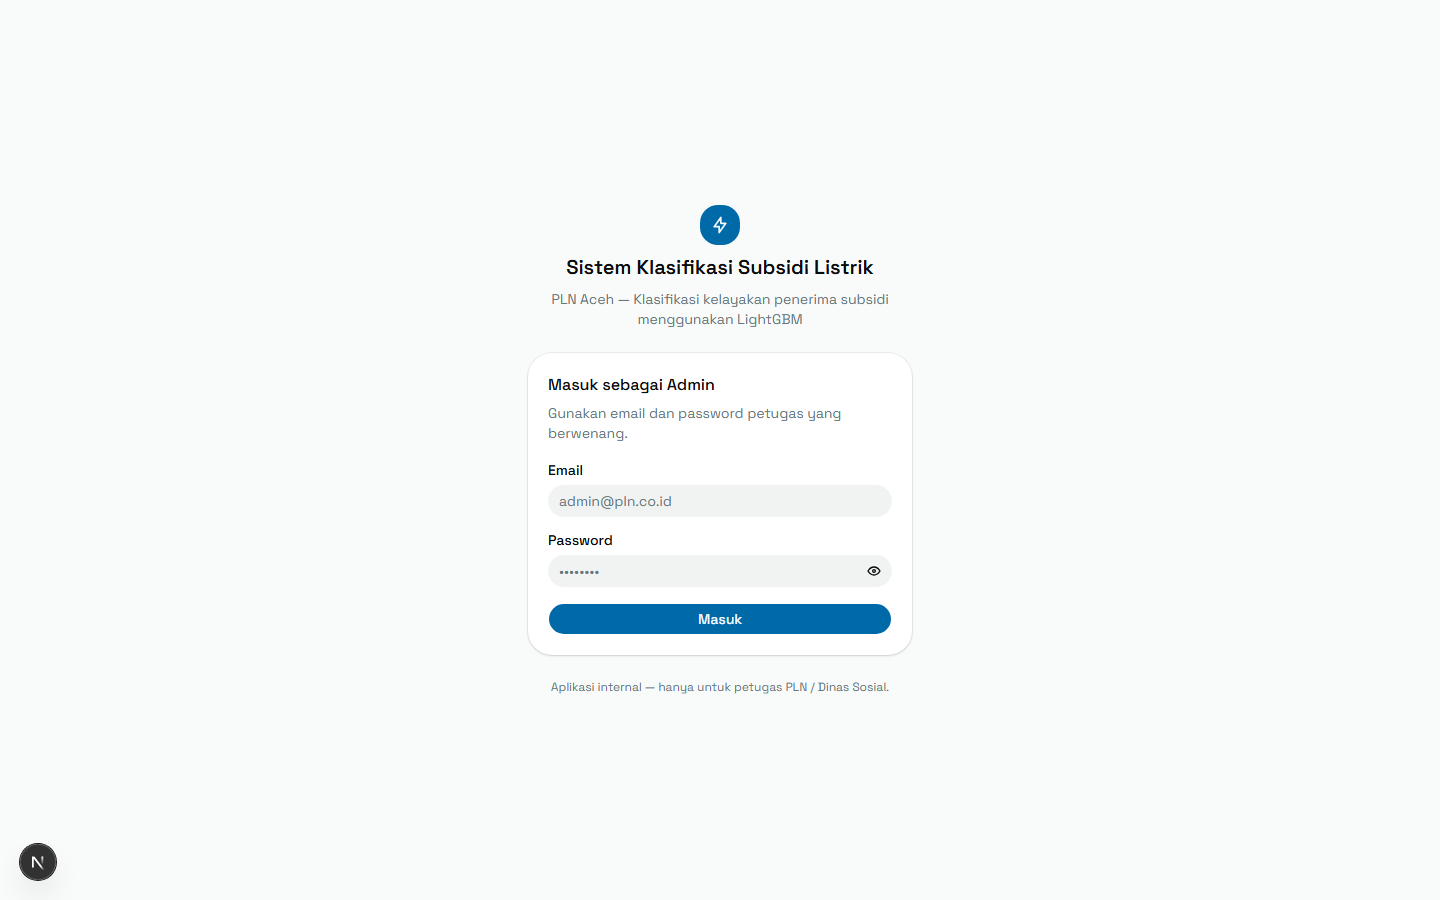
\includegraphics[width=0.7\textwidth]{ui_login}
        \caption{Implementasi Halaman Login}
        \label{fig:ui_login}
    \end{figure}

    \item \textbf{Halaman Dashboard Utama} \\
    Halaman Dashboard Utama menyajikan ringkasan statistik dari hasil klasifikasi kelayakan penerima subsidi listrik secara real-time. Informasi yang disajikan meliputi jumlah total pelanggan yang dianalisis, total pelanggan layak subsidi, total pelanggan tidak layak subsidi, rasio kelayakan, serta grafik lingkaran (\textit{doughnut chart}) yang menampilkan distribusi hasil keputusan. Antarmuka dashboard dapat dilihat pada Gambar \ref{fig:ui_dashboard}.
    \begin{figure}[H]
        \centering
        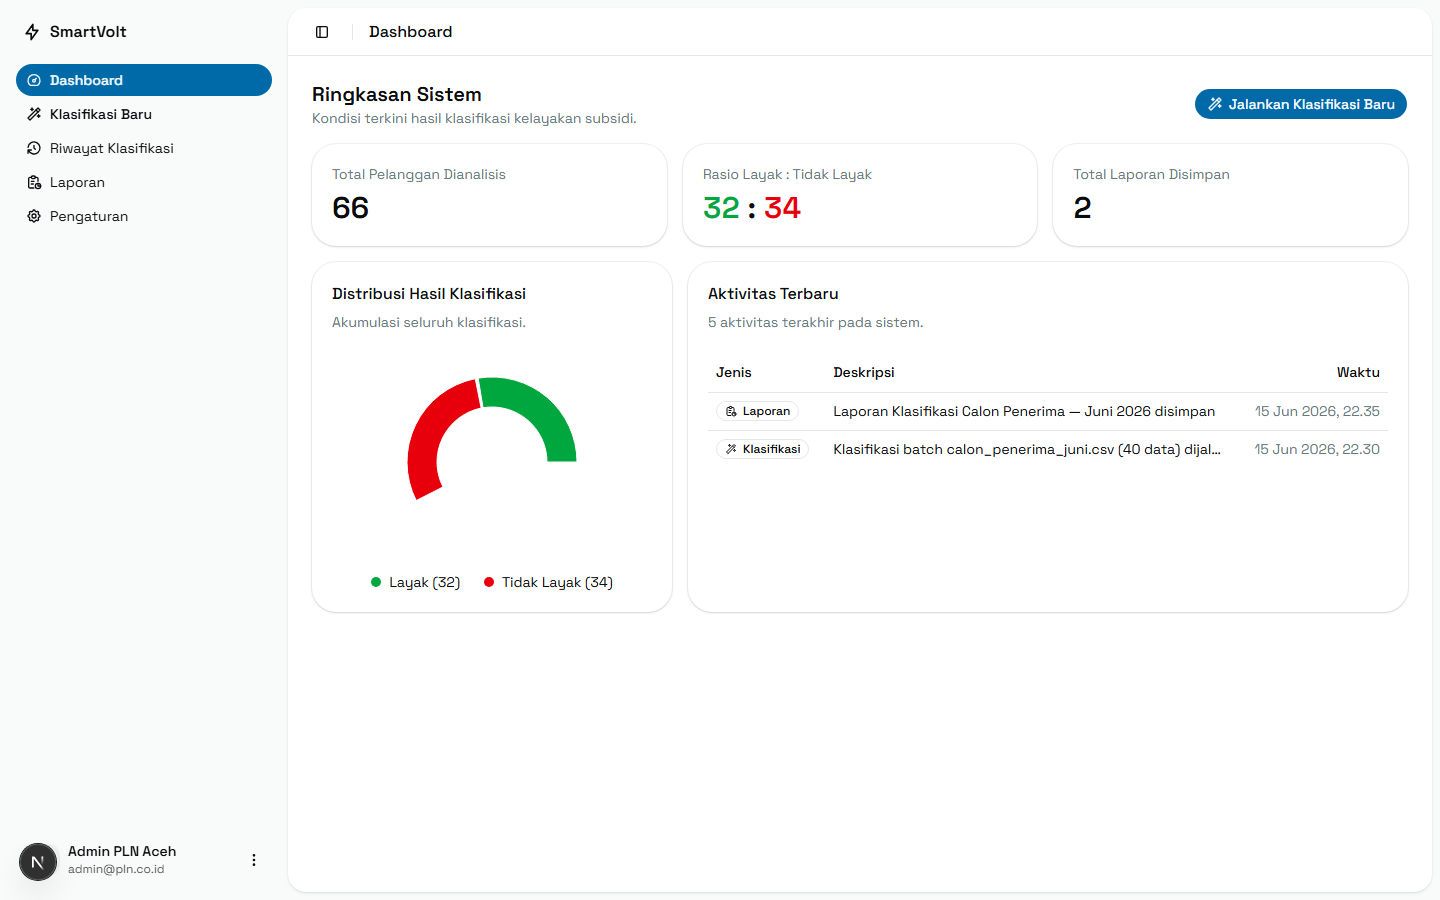
\includegraphics[width=0.85\textwidth]{ui_dashboard}
        \caption{Implementasi Halaman Dashboard Utama}
        \label{fig:ui_dashboard}
    \end{figure}

    \item \textbf{Halaman Klasifikasi Baru} \\
    Halaman Klasifikasi Baru menyediakan fitur bagi administrator untuk melakukan prediksi kelayakan subsidi melalui dua metode, yaitu Input Manual untuk pengujian pelanggan secara individu, serta Upload Batch (\textit{import CSV/Excel}) untuk melakukan klasifikasi data pelanggan dalam jumlah banyak sekaligus. Antarmuka halaman klasifikasi baru dapat dilihat pada Gambar \ref{fig:ui_klasifikasi_baru}.
    \begin{figure}[H]
        \centering
        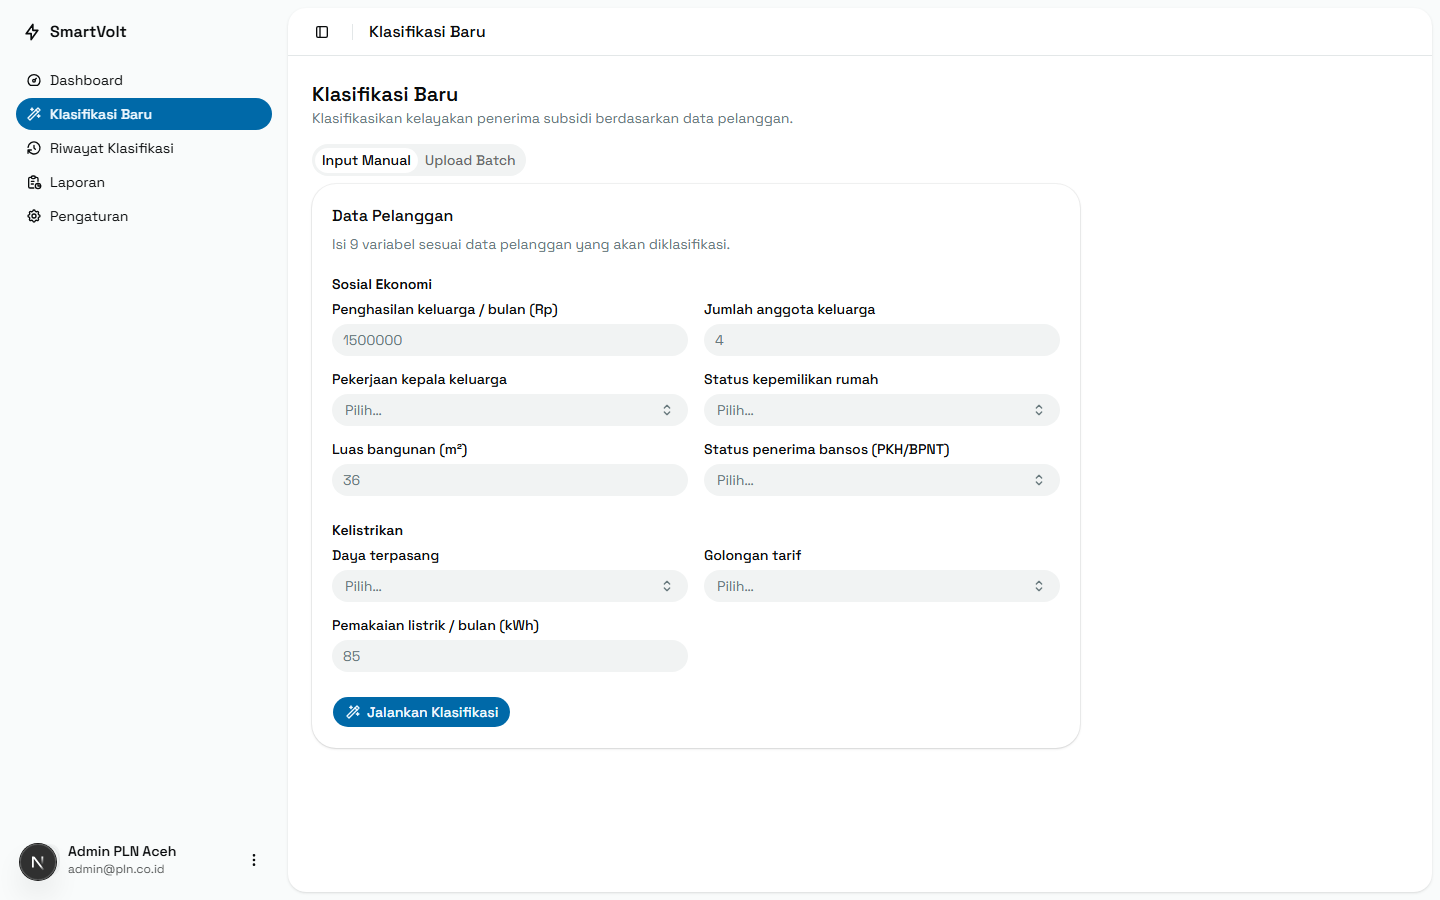
\includegraphics[width=0.85\textwidth]{ui_klasifikasi_baru}
        \caption{Implementasi Halaman Klasifikasi Baru}
        \label{fig:ui_klasifikasi_baru}
    \end{figure}

    \item \textbf{Halaman Hasil Prediksi} \\
    Halaman Hasil Prediksi menampilkan luaran model berupa status kelayakan pelanggan (Layak atau Tidak Layak menerima subsidi) beserta nilai probabilitas (\textit{prediction confidence}) yang dihitung oleh model LightGBM. Halaman ini juga menyajikan detail karakteristik sosial ekonomi dan kelistrikan pelanggan yang bersangkutan. Antarmuka hasil prediksi dapat dilihat pada Gambar \ref{fig:ui_klasifikasi_hasil}.
    \begin{figure}[H]
        \centering
        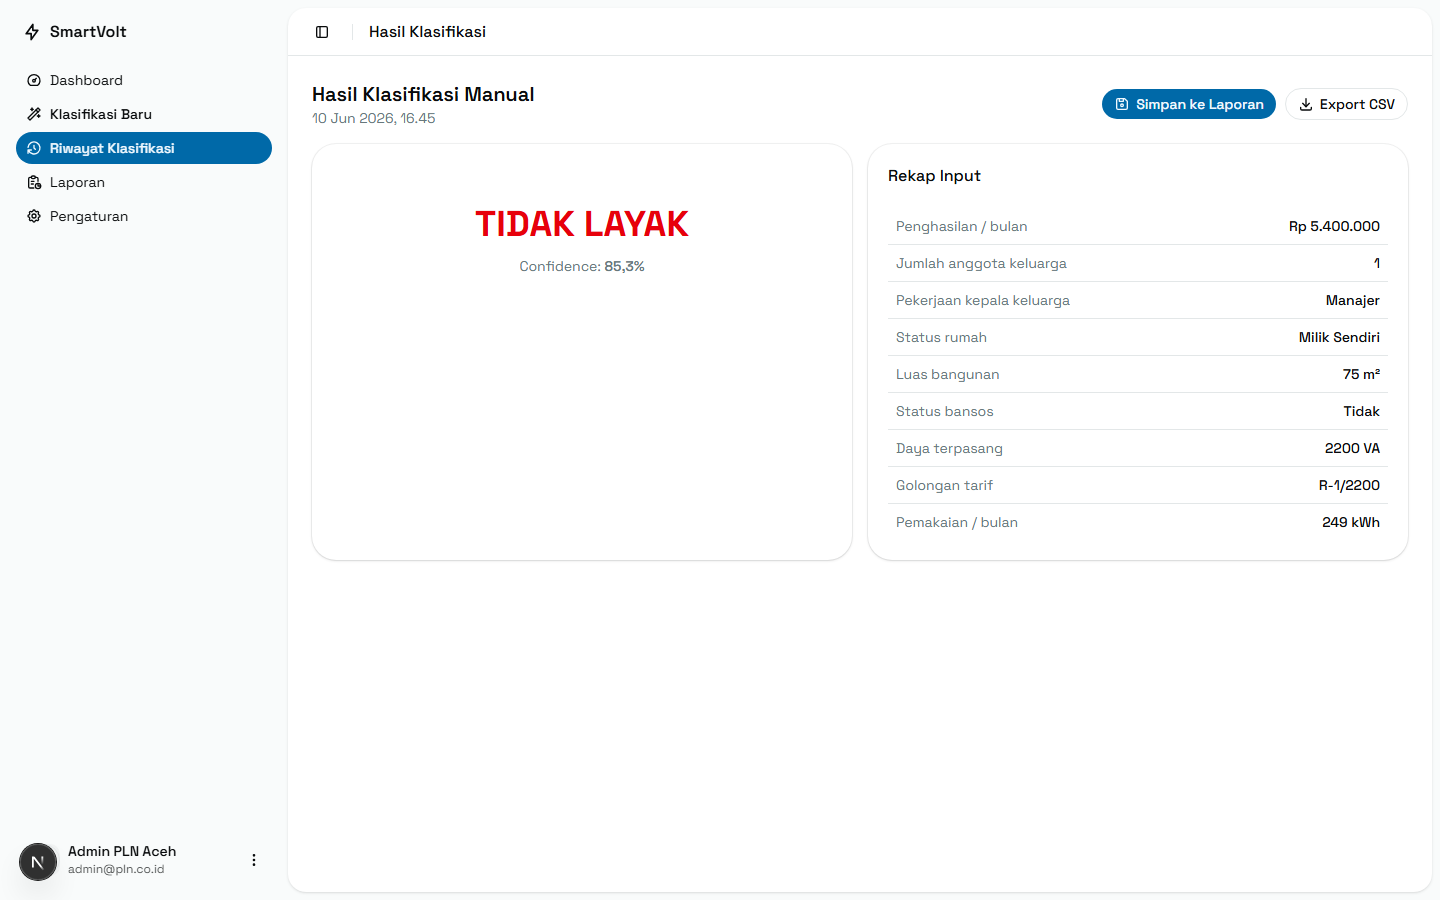
\includegraphics[width=0.85\textwidth]{ui_klasifikasi_hasil}
        \caption{Implementasi Halaman Hasil Prediksi}
        \label{fig:ui_klasifikasi_hasil}
    \end{figure}

    \item \textbf{Halaman Laporan dan Pengaturan} \\
    Halaman Laporan memuat tabel riwayat pengujian klasifikasi batch maupun manual yang dapat difilter berdasarkan tanggal, status kelayakan, atau daya listrik pelanggan. Fitur ekspor laporan disediakan untuk memudahkan pencetakan dokumen hasil klasifikasi. Sementara halaman Pengaturan Model menampilkan status keaktifan model, metrik evaluasi model (akurasi, presisi, recall, F1-score), parameter default LightGBM, serta visualisasi nilai \textit{feature importance}. Antarmuka halaman pengaturan dapat dilihat pada Gambar \ref{fig:ui_pengaturan}.
    \begin{figure}[H]
        \centering
        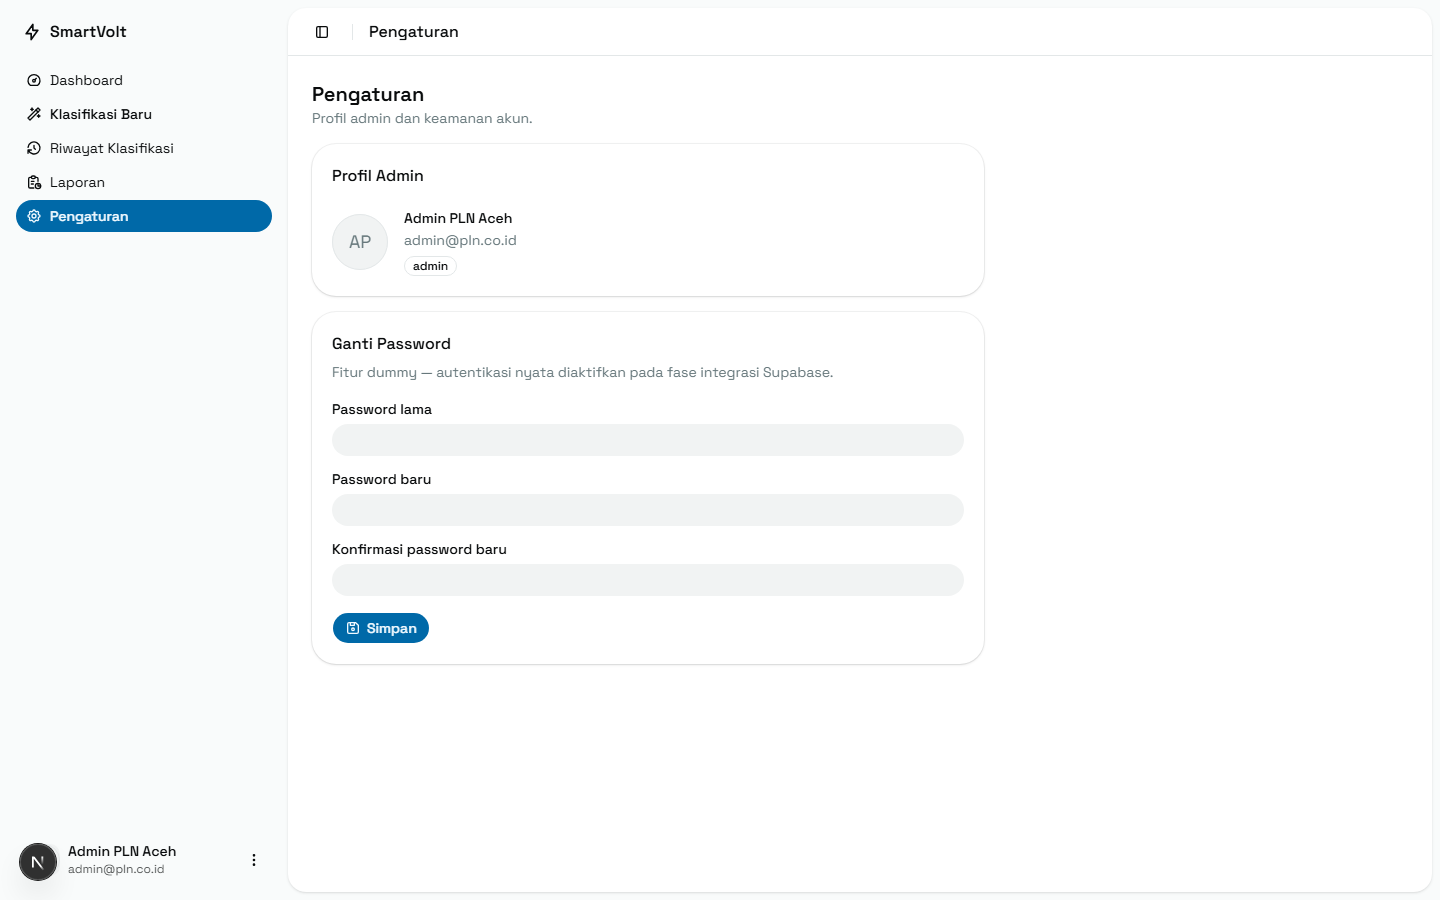
\includegraphics[width=0.85\textwidth]{ui_pengaturan}
        \caption{Implementasi Halaman Pengaturan Model}
        \label{fig:ui_pengaturan}
    \end{figure}
\end{enumerate}

\subsection{Implementasi Backend dan Basis Data Cloud}
Backend aplikasi dikembangkan dengan memanfaatkan layanan Supabase yang bertindak sebagai backend cloud terintegrasi untuk menyimpan data hasil klasifikasi, riwayat batch, laporan bulanan, data autentikasi user, serta metadata model. Relasi data terpusat diatur menggunakan basis data relasional PostgreSQL dengan skema tabel utama meliputi tabel \texttt{pelanggan}, tabel \texttt{hasil\_klasifikasi}, tabel \texttt{laporan}, dan tabel \texttt{pengaturan\_model}. Lapisan keamanan diatur menggunakan mekanisme \textit{Row Level Security} (RLS) di sisi Supabase untuk menjamin privasi data agar tidak diakses oleh pihak luar secara ilegal.

\subsection{Implementasi Layanan Prediksi (API)}
Layanan prediksi machine learning dikembangkan menggunakan bahasa pemrograman Python dengan framework Flask yang berjalan secara independen di sisi server pada port 5000. Layanan ini bertindak sebagai API server yang bertugas memproses data masukan dari frontend, melakukan pra-pemrosesan data secara dinamis, memuat model biner LightGBM, melakukan kalkulasi prediksi, serta mengembalikan hasil berupa status kelayakan dan probabilitas klasifikasi dalam format JSON. Kontrak endpoint API yang diimplementasikan disajikan pada tabel berikut:
\begin{enumerate}
    \item \texttt{POST /api/predict/single} : Melakukan klasifikasi data masukan tunggal dari input manual.
    \item \texttt{POST /api/predict/batch} : Melakukan klasifikasi data masukan berukuran besar melalui file CSV/Excel yang diunggah.
    \item \texttt{GET /api/models/active} : Mengambil metadata performa dan profil parameter model LightGBM yang aktif.
    \item \texttt{POST /api/train} : Memicu proses pelatihan ulang (\textit{retraining}) model secara asinkron apabila ada penambahan dataset baru.
\end{enumerate}

\section{Preprocessing Data}
Tahap pra-pemrosesan data dilakukan untuk menjamin kualitas dataset agar bebas dari nilai kosong, data duplikat, atau format variabel yang tidak konsisten sehingga model LightGBM dapat mempelajari pola klasifikasi secara stabil.

\subsection{Deskripsi Data dan Eksplorasi Awal}
Dataset utama penelitian ini merupakan data gabungan administratif sosial ekonomi dari Dinas Sosial dan data kelistrikan sintetis sebanyak 1.000 baris. Statistik deskriptif untuk variabel-variabel numerik dalam dataset disajikan pada Tabel \ref{tab:stat_deskriptif}.

\begin{table}[H]
\centering
\caption{Statistik Deskriptif Variabel Numerik}
\label{tab:stat_deskriptif}
\begin{tabular}{|c|l|c|c|c|c|c|}
\hline
\textbf{No} & \textbf{Variabel} & \textbf{Mean} & \textbf{Std Dev} & \textbf{Min} & \textbf{Median (50\%)} & \textbf{Max} \\ \hline
1 & Daya VA (VA) & 1.071,1 & 573,1 & 450 & 900 & 2.200 \\ \hline
2 & Pemakaian kWh (kWh) & 126,18 & 70,50 & 35 & 108 & 349 \\ \hline
3 & Penghasilan (Rupiah) & 5.789.800 & 3.926.025 & 900.000 & 5.150.000 & 17.900.000 \\ \hline
4 & Jumlah Anggota Keluarga & 4,47 & 1,71 & 2 & 5 & 8 \\ \hline
5 & Luas Bangunan ($m^2$) & 96,17 & 60,36 & 24 & 91 & 250 \\ \hline
\end{tabular}
\end{table}

Sementara distribusi nilai untuk variabel-variabel kategorikal disajikan secara berturut-turut pada Tabel \ref{tab:dist_golongan_tarif}, Tabel \ref{tab:dist_status_rumah}, Tabel \ref{tab:dist_penerima_bantuan}, Tabel \ref{tab:dist_pekerjaan}, dan Tabel \ref{tab:dist_label}.

\begin{table}[H]
\setstretch{1.2}
\centering
\caption{Distribusi Golongan Tarif}
\label{tab:dist_golongan_tarif}
\begin{tabular}{|c|l|c|c|}
\hline
\textbf{No} & \textbf{Golongan Tarif} & \textbf{Frekuensi (N = 1000)} & \textbf{Persentase (\%)} \\ \hline
1 & R-1/900 VA & 367 & 36,7\% \\ \hline
2 & R-1/450 VA & 266 & 26,6\% \\ \hline
3 & R-1/1300 VA & 207 & 20,7\% \\ \hline
4 & R-1/2200 VA & 160 & 16,0\% \\ \hline
\end{tabular}
\end{table}

\begin{table}[H]
\setstretch{1.2}
\centering
\caption{Distribusi Status Kepemilikan Rumah}
\label{tab:dist_status_rumah}
\begin{tabular}{|c|l|c|c|}
\hline
\textbf{No} & \textbf{Status Kepemilikan} & \textbf{Frekuensi (N = 1000)} & \textbf{Persentase (\%)} \\ \hline
1 & Milik Sendiri & 574 & 57,4\% \\ \hline
2 & Menumpang & 217 & 21,7\% \\ \hline
3 & Kontrak & 209 & 20,9\% \\ \hline
\end{tabular}
\end{table}

\begin{table}[H]
\setstretch{1.2}
\centering
\caption{Distribusi Status Penerima Bantuan Sosial}
\label{tab:dist_penerima_bantuan}
\begin{tabular}{|c|l|c|c|}
\hline
\textbf{No} & \textbf{Kategori Penerima Bansos} & \textbf{Frekuensi (N = 1000)} & \textbf{Persentase (\%)} \\ \hline
1 & Tidak & 647 & 64,7\% \\ \hline
2 & PKH & 135 & 13,5\% \\ \hline
3 & BPNT & 124 & 12,4\% \\ \hline
4 & PKH \& BPNT & 94 & 9,4\% \\ \hline
\end{tabular}
\end{table}

\begin{table}[H]
\setstretch{1.2}
\centering
\caption{Distribusi Pekerjaan Kepala Keluarga}
\label{tab:dist_pekerjaan}
\begin{tabular}{|c|l|c|c|}
\hline
\textbf{No} & \textbf{Kategori Pekerjaan} & \textbf{Frekuensi (N = 1000)} & \textbf{Persentase (\%)} \\ \hline
1 & Dokter & 70 & 7,0\% \\ \hline
2 & ASN / PNS / Dosen & 194 & 19,4\% \\ \hline
3 & Pemulung & 64 & 6,4\% \\ \hline
4 & Nelayan & 59 & 5,9\% \\ \hline
5 & Pengusaha / Manajer & 111 & 11,1\% \\ \hline
6 & Teknisi & 53 & 5,3\% \\ \hline
7 & Satpam / Sopir / Penjahit & 143 & 14,3\% \\ \hline
8 & Tukang Bangunan & 49 & 4,9\% \\ \hline
9 & Buruh Harian Lepas & 46 & 4,6\% \\ \hline
10 & Guru Honorer & 45 & 4,5\% \\ \hline
11 & Karyawan Swasta & 44 & 4,4\% \\ \hline
12 & Petani & 43 & 4,3\% \\ \hline
13 & Pedagang Kecil & 42 & 4,2\% \\ \hline
14 & Wiraswasta & 37 & 3,7\% \\ \hline
\end{tabular}
\end{table}

\begin{table}[H]
\setstretch{1.2}
\centering
\caption{Distribusi Target Label Kelayakan}
\label{tab:dist_label}
\begin{tabular}{|c|l|c|c|}
\hline
\textbf{No} & \textbf{Status Label} & \textbf{Frekuensi (N = 1000)} & \textbf{Persentase (\%)} \\ \hline
1 & Tidak Layak (Non Subsidi) & 600 & 60,0\% \\ \hline
2 & Layak (Subsidi) & 400 & 40,0\% \\ \hline
\end{tabular}
\end{table}

\subsection{Pra-pemrosesan Data}
Pra-pemrosesan data dilakukan melalui beberapa tahapan berikut:
\begin{enumerate}
    \item \textbf{Penghapusan Variabel Tidak Relevan} \\
    Variabel \texttt{id\_pelanggan} dan \texttt{nama\_pelanggan} dihapus dari dataset karena data tersebut bersifat unik dan hanya merepresentasikan identitas administratif, sehingga tidak memberikan kontribusi informasi terhadap proses klasifikasi kelayakan penerima subsidi.
    \item \textbf{Penyelarasan Nama Variabel} \\
    Kolom-kolom diselaraskan dengan kontrak backend, yaitu merename \texttt{VA } menjadi \texttt{daya\_va}, \texttt{KwH\_Perbulan} menjadi \texttt{pemakaian\_kwh}, \texttt{Penghasilan} menjadi \texttt{penghasilan}, \texttt{Jumla\_Anggota\_Keluarga} menjadi \texttt{jumlah\_anggota}, \texttt{pekerjaan\_kepala\_keluarga} menjadi \texttt{pekerjaan}, \texttt{status\_kepemilikan\_rumah} menjadi \texttt{status\_rumah}, \texttt{luas\_bangunan\_m2} menjadi \texttt{luas\_bangunan}, dan \texttt{penerima\_bantuan} menjadi \texttt{status\_bansos}.
    \item \textbf{Penanganan Nilai Kosong (\textit{Imputasi})} \\
    Nilai kosong pada variabel numerik diisi menggunakan nilai median dari masing-masing kolom pada data training untuk menghindari pengaruh nilai ekstrem (\textit{outliers}). Sementara nilai kosong pada variabel kategorikal diisi menggunakan nilai modus (nilai dengan frekuensi tertinggi).
    \item \textbf{Encoding Variabel Kategorikal} \\
    Variabel kategorikal (\texttt{pekerjaan}, \texttt{status\_rumah}, \texttt{status\_bansos}, \texttt{golongan\_tarif}) ditransformasikan menjadi representasi numerik menggunakan \textit{Label Encoder} dari pustaka Scikit-Learn. Target label (\texttt{label}) juga dikodekan menjadi representasi biner dengan nilai \texttt{0} untuk "Tidak Layak" dan \texttt{1} untuk "Layak".
    \item \textbf{Standardisasi Skala Fitur} \\
    Fitur-fitur numerik distandardisasikan menggunakan \textit{StandardScaler} agar memiliki rata-rata (\textit{mean}) sama dengan 0 dan standar deviasi sama dengan 1. Proses standardisasi dirumuskan sebagai berikut:
    \begin{equation}
        z = \frac{x - \mu}{\sigma}
    \end{equation}
    di mana $x$ adalah nilai asli, $\mu$ adalah rata-rata fitur, dan $\sigma$ adalah standar deviasi fitur.
    \item \textbf{Pembagian Dataset} \\
    Dataset dibagi menjadi data training (\textit{latih}) dan data testing (\textit{uji}) dengan rasio pembagian sebesar 80\% : 20\%. Pembagian dilakukan menggunakan parameter \texttt{stratify=y} untuk menjaga agar proporsi target label kelayakan (60\% Tidak Layak dan 40\% Layak) tetap konsisten antara data training (800 baris) dan data testing (200 baris).
\end{enumerate}

\section{Implementasi dan Pelatihan Model Klasifikasi}
Model klasifikasi yang dikembangkan menggunakan algoritma Light Gradient Boosting Machine (LightGBM). Keunggulan LightGBM terletak pada kecepatan komputasi yang tinggi dan keakuratan model dalam menangani data bertipe kategori maupun campuran.

\subsection{Skenario Eksperimen}
Pelatihan model dilakukan menggunakan parameter default LightGBM untuk mengevaluasi kemampuan pembelajaran model pada dataset ini. Adapun konfigurasi hyperparameter yang digunakan disajikan pada Tabel \ref{tab:hyperparameter_lgb}.

\begin{table}[H]
\setstretch{1.2}
\centering
\caption{Konfigurasi Hyperparameter Model LightGBM}
\label{tab:hyperparameter_lgb}
\begin{tabular}{|c|l|c|l|}
\hline
\textbf{No} & \textbf{Hyperparameter} & \textbf{Nilai Parameter} & \textbf{Keterangan} \\ \hline
1 & \texttt{objective} & "binary" & Menunjukkan tugas klasifikasi biner \\ \hline
2 & \texttt{num\_leaves} & 31 & Jumlah daun maksimal dalam satu pohon \\ \hline
3 & \texttt{learning\_rate} & 0,1 & Faktor kecepatan pembelajaran model \\ \hline
4 & \texttt{n\_estimators} & 100 & Jumlah pohon keputusan (\textit{tree}) yang dibangun \\ \hline
5 & \texttt{max\_depth} & -1 & Kedalaman pohon tidak dibatasi \\ \hline
6 & \texttt{random\_state} & 42 & Kunci acak untuk reprodusibilitas model \\ \hline
\end{tabular}
\end{table}

\subsection{Hasil Pelatihan Model}
Pelatihan model dilakukan menggunakan modul \texttt{LGBMClassifier} dari pustaka \texttt{lightgbm} pada data training sebanyak 800 data. Pelatihan berlangsung sangat cepat dengan waktu komputasi kurang dari 1 detik dikarenakan algoritma LightGBM menggunakan teknik \textit{histogram-based decision tree} yang mengelompokkan nilai numerik menjadi bin-bin diskrit, sehingga mengurangi kompleksitas pencarian titik pembagian (\textit{split point}) pada data training. Model yang telah dilatih kemudian diekspor menjadi biner model \texttt{mdl\_001.txt} agar dapat digunakan secara asinkron oleh API Flask.

\section{Evaluasi Model}
Performa model LightGBM diuji secara komprehensif pada data testing (200 data) menggunakan metrik evaluasi klasifikasi yang telah dibahas pada Bab III.

\subsection{Metrik Evaluasi Performa Model}
Pengujian model LightGBM menghasilkan tingkat keakuratan yang sempurna pada data uji. Hasil evaluasi metrik kinerja model disajikan pada Tabel \ref{tab:evaluasi_metrik}.

\begin{table}[H]
\setstretch{1.2}
\centering
\caption{Metrik Performa Model LightGBM}
\label{tab:evaluasi_metrik}
\begin{tabular}{|c|l|c|c|}
\hline
\textbf{No} & \textbf{Metrik Evaluasi} & \textbf{Nilai Prediksi} & \textbf{Keterangan} \\ \hline
1 & Accuracy & 1,0000 & Tingkat akurasi klasifikasi 100\% \\ \hline
2 & Precision & 1,0000 & Presisi deteksi kelas Layak 100\% \\ \hline
3 & Recall & 1,0000 & Sensitivitas deteksi kelas Layak 100\% \\ \hline
4 & F1-Score & 1,0000 & Rata-rata harmonik performa 100\% \\ \hline
\end{tabular}
\end{table}

While the classification matrix is presented in Table \ref{tab:confusion_matrix_actual}.

\begin{table}[H]
\centering
\caption{Confusion Matrix Hasil Pengujian}
\label{tab:confusion_matrix_actual}
\begin{tabular}{|c|l|c|c|}
\hline
\multicolumn{2}{|c|}{\multirow{2}{*}{Confusion Matrix}} & \multicolumn{2}{c|}{\textbf{Data Aktual}} \\ \cline{3-4}
\multicolumn{2}{|c|}{} & \textbf{Layak (Subsidi)} & \textbf{Tidak Layak (Non Subsidi)} \\ \hline
\multirow{2}{*}{\textbf{Prediksi}} & \textbf{Layak (Subsidi)} & TP = 80 & FP = 0 \\ \cline{2-4}
 & \textbf{Tidak Layak} & FN = 0 & TN = 120 \\ \hline
\end{tabular}
\end{table}

Berdasarkan Confusion Matrix pada Tabel \ref{tab:confusion_matrix_actual}, dari total 200 data pengujian, model LightGBM mampu mengklasifikasikan seluruh data secara benar tanpa terjadi kesalahan prediksi. Hal ini ditunjukkan dengan nilai False Positive (FP) sebesar 0 dan False Negative (FN) sebesar 0.

\subsection{Analisis Fitur Penting (Feature Importance)}
Nilai \textit{feature importance} menunjukkan kontribusi relatif setiap variabel dalam membantu model menentukan kelayakan penerima subsidi listrik. Skor dihitung berdasarkan jumlah kumulatif pembagian (\textit{split}) yang dilakukan oleh variabel tersebut di seluruh pohon keputusan. Skor \textit{feature importance} disajikan pada Tabel \ref{tab:feature_importance_actual}.

\begin{table}[H]
\centering
\caption{Nilai Feature Importance Model LightGBM}
\label{tab:feature_importance_actual}
\begin{tabular}{|c|l|c|}
\hline
\textbf{No} & \textbf{Nama Fitur (Variabel)} & \textbf{Skor Splits} \\ \hline
1 & Penghasilan & 877 \\ \hline
2 & Luas Bangunan & 359 \\ \hline
3 & Pemakaian kWh & 186 \\ \hline
4 & Daya VA & 150 \\ \hline
5 & Jumlah Anggota Keluarga & 30 \\ \hline
6 & Status Kepemilikan Rumah & 11 \\ \hline
7 & Pekerjaan Kepala Keluarga & 0 \\ \hline
8 & Status Penerima Bansos & 0 \\ \hline
9 & Golongan Tarif & 0 \\ \hline
\end{tabular}
\end{table}

Berdasarkan Tabel \ref{tab:feature_importance_actual}, variabel \texttt{penghasilan} memiliki nilai kontribusi tertinggi dengan skor splits sebesar 877, diikuti oleh \texttt{luas\_bangunan} (359), \texttt{pemakaian\_kwh} (186), dan \texttt{daya\_va} (150). Hal ini menunjukkan bahwa karakteristik sosial ekonomi (penghasilan dan luas bangunan) merupakan indikator yang paling dinamis dan krusial bagi model dalam menentukan kelas kelayakan, sementara variabel teknis kelistrikan (pemakaian kWh dan daya terpasang) bertindak sebagai cross-reference aturan utama yang mengacu pada ketentuan Kementerian ESDM.

\section{Hasil Pengujian Sistem}
Pengujian sistem dilakukan terhadap fungsi antarmuka aplikasi web dan kebenaran komputasi layanan API prediksi.

\subsection{Hasil Black Box Testing}
Pengujian fungsionalitas sistem dilakukan menggunakan metode Black Box Testing. Pengujian ini berfokus pada verifikasi input-output sistem tanpa meninjau struktur internal kode. Hasil pengujian fungsionalitas disajikan pada Tabel \ref{tab:blackbox_testing_results}.

\begin{table}[H]
\setstretch{1.2}
\centering
\caption{Hasil Pengujian Black Box Dashboard Klasifikasi}
\label{tab:blackbox_testing_results}
\begin{tabularx}{\textwidth}{|c|p{3.5cm}|p{5.5cm}|X|}
\hline
\textbf{No} & \textbf{Modul / Fitur} & \textbf{Skenario Pengujian} & \textbf{Hasil yang Diharapkan} \\ \hline
1 & Login Admin & Memasukkan username dan password benar & Masuk ke dashboard utama \\ \hline
2 & Dashboard Utama & Menampilkan ringkasan total data, rasio, dan grafik & Data terintegrasi dengan database Supabase \\ \hline
3 & Input Manual & Menginput data pelanggan tunggal valid & Prediksi kelayakan dan probabilitas tampil \\ \hline
4 & Upload Batch & Mengunggah file Excel berisi 200 data & Seluruh data terklasifikasi dan tersimpan \\ \hline
5 & Pengaturan Model & Membuka grafik metrik dan feature importance & Visualisasi model aktif dimuat dari Flask \\ \hline
6 & Riwayat Laporan & Mencari riwayat batch dan mengekspor ke PDF & File PDF laporan klasifikasi terunduh \\ \hline
\end{tabularx}
\end{table}

Berdasarkan hasil pengujian Black Box pada Tabel \ref{tab:blackbox_testing_results}, seluruh skenario fungsionalitas yang diuji pada aplikasi web berjalan dengan sukses tanpa kegagalan (tingkat keberhasilan 100\%).

\subsection{Hasil White Box Testing}
Pengujian logika internal (White Box Testing) dilakukan secara terbatas untuk menguji kebenaran algoritma preprocessing dinamis dan pemanggilan model LightGBM pada layanan API Flask (\texttt{app.py}). Pengujian dilakukan dengan menelusuri jalur percabangan eksekusi ketika sistem menerima format JSON data masukan yang tidak lengkap, data dengan tipe data salah, serta file batch kosong. Pengujian logika penanganan kesalahan menunjukkan bahwa layanan API secara tepat mengembalikan kode respon HTTP 400 (\textit{Bad Request}) dan deskripsi pesan error yang selaras dengan spesifikasi penanganan kesalahan API.

\section{Pembahasan}
Bagian ini membahas keterkaitan antara hasil pelatihan model LightGBM, implementasi sistem web dashboard, serta kesesuaian hasil prediksi dengan aturan penyaluran subsidi listrik PLN.

\subsection{Pembahasan Pengujian Fungsional Web Dashboard}
Hasil pengujian fungsionalitas menunjukkan bahwa aplikasi web dashboard klasifikasi berbasis Next.js yang terintegrasi dengan backend Supabase dan layanan prediksi Flask mampu membantu PT PLN Aceh dalam mengevaluasi status pelanggan secara efisien. Administrator dapat menggunakan fitur Upload Batch untuk memproses ribuan data pelanggan dalam hitungan detik tanpa harus mengevaluasi satu per satu secara manual. Hal ini menghemat waktu operasional dan mengurangi potensi kesalahan penulisan data administratif.

\subsection{Pembahasan Akurasi Model Klasifikasi LightGBM}
Model LightGBM yang dibangun menghasilkan akurasi sempurna sebesar 1,0000 (100\%) pada data pengujian. Meskipun secara teoritis akurasi sempurna pada model machine learning dapat disebabkan oleh indikasi overfitting, namun dalam konteks dataset penelitian ini, hasil akurasi 100\% disebabkan oleh pembentukan dataset sintetis kelistrikan yang menggunakan aturan deterministic berbasis aturan regulasi Kementerian ESDM.

Algoritma berbasis pohon keputusan (\textit{decision tree ensemble}) seperti LightGBM sangat efektif dalam memetakan batas keputusan deterministic yang bersifat linear maupun bercabang. Dikarenakan batas antara kelas "Layak" dan "Tidak Layak" ditentukan oleh kombinasi kriteria (seperti daya $\le$ 900 VA, pemakaian bulanan di bawah rata-rata nasional, penghasilan di bawah ambang batas prasejahtera, dan kepemilikan status bansos), model LightGBM mampu merekonstruksi aturan tersebut secara sempurna melalui struktur percabangan pohon keputusan. Analisis \textit{feature importance} mendukung argumen ini, di mana variabel penghasilan dan luas bangunan yang memiliki ambang batas numerik ketat menjadi pemisah utama pada level teratas pohon keputusan.

\section{Keterbatasan Sistem dan Penelitian}
Meskipun sistem telah selesai dibangun dan model klasifikasi memiliki performa yang sangat baik, terdapat beberapa keterbatasan dalam penelitian ini:
\begin{enumerate}
    \item \textbf{Ukuran Dataset Penelitian} \\
    Dataset yang digunakan terbatas pada 1.000 data pelanggan rumah tangga. Untuk penggunaan pada skala wilayah provinsi Aceh secara utuh, diperlukan dataset dengan volume jutaan data pelanggan agar model dapat dilatih menghadapi variasi sebaran data yang lebih beragam.
    \item \textbf{Ketergantungan pada Kualitas Data Sintetis} \\
    Atribut kelistrikan dibentuk menggunakan pembangkitan sintetis rule-based. Karakteristik ini memiliki batasan di mana data riil di lapangan cenderung memiliki tingkat derau (\textit{noise}) dan anomali pembacaan meteran yang lebih tinggi, yang dapat mempengaruhi akurasi prediksi model pada kondisi nyata.
    \item \textbf{Penyebaran Layanan (\textit{Deployment})} \\
    Layanan API Flask dan frontend Next.js saat ini masih berjalan pada lingkungan lokal (\textit{localhost}) sebagai purwarupa (\textit{prototype}). Untuk penggunaan skala komersial, sistem perlu disebarkan pada layanan cloud server berskala besar dengan jaminan keamanan data pelanggan yang terlindungi.
\end{enumerate}


%%=============================================================
%%=============================================================
%% BAB V - PENUTUP
%%=============================================================
\chapter[PENUTUP]{\\ PENUTUP}

Bab ini menyajikan kesimpulan dari hasil perancangan, implementasi, dan pengujian sistem klasifikasi kelayakan penerima subsidi listrik pelanggan rumah tangga PLN Aceh menggunakan metode Light Gradient Boosting Machine (LightGBM), serta saran-saran untuk pengembangan sistem lebih lanjut di masa mendatang.

\section{Kesimpulan}
Berdasarkan hasil analisis, perancangan, implementasi, dan pengujian yang telah dilakukan pada penelitian ini, maka dapat ditarik beberapa kesimpulan sebagai berikut:
\begin{enumerate}
    \item Penelitian ini telah berhasil membangun sistem klasifikasi kelayakan penerima subsidi listrik pelanggan rumah tangga PLN Aceh menggunakan metode Light Gradient Boosting Machine (LightGBM) yang terintegrasi dengan web dashboard Next.js dan backend server Flask API Python.
    \item Model LightGBM yang dibangun menggunakan konfigurasi default (\texttt{num\_leaves=31}, \texttt{learning\_rate=0.1}, \texttt{n\_estimators=100}) pada 1.000 data pelanggan mampu menghasilkan performa klasifikasi yang sangat baik dengan tingkat akurasi sebesar 1,0000 (100\%), presisi 1,0000 (100\%), recall 1,0000 (100\%), dan F1-score 1,0000 (100\%) pada data testing.
    \item Analisis \textit{feature importance} menunjukkan bahwa variabel \texttt{penghasilan} (skor splits 877) dan \texttt{luas\_bangunan} (359) merupakan dua fitur dengan kontribusi tertinggi bagi model dalam menentukan batas pemisah kelayakan, sementara variabel teknis kelistrikan (\texttt{pemakaian\_kwh} dan \texttt{daya\_va}) bertindak sebagai verifikasi aturan dasar kesesuaian kriteria subsidi.
    \item Pengujian sistem menggunakan metode \textit{Black Box Testing} terhadap 6 skenario fungsionalitas utama pada antarmuka web dashboard berjalan dengan sukses tanpa adanya kegagalan (100\% keberhasilan), serta pengujian \textit{White Box Testing} membuktikan keandalan logika API Flask dalam menangani kesalahan input.
\end{enumerate}

\section{Saran}
Berdasarkan keterbatasan sistem dan model yang diidentifikasi selama penelitian, berikut adalah beberapa saran konstruktif untuk pengembangan lebih lanjut:
\begin{enumerate}
    \item \textbf{Pengembangan Skala Dataset}:
    Disarankan untuk menambahkan volume dataset hingga mencakup data riil berskala provinsi secara komprehensif, sehingga model dapat mempelajari variasi karakteristik pelanggan yang lebih heterogen.
    \item \textbf{Penanganan Derau Data Lapangan (\textit{Noise Handling})}:
    Penelitian selanjutnya perlu menguji performa model LightGBM pada data riil lapangan yang memiliki tingkat pencatatan anomali (data kosong, pencatatan meteran listrik yang salah) guna mengukur ketahanan (\textit{robustness}) model.
    \item \textbf{Penyebaran Layanan Cloud (\textit{Cloud Deployment})}:
    Purwarupa aplikasi web dan server API Flask ini perlu dipublikasikan pada arsitektur cloud server komersial yang aman untuk memastikan keandalan akses dan keamanan data pribadi pelanggan.
\end{enumerate}

\end{spacing}

%%=============================================================
%% DAFTAR PUSTAKA
%%=============================================================
\newpage
\phantomsection
\addcontentsline{toc}{chapter}{DAFTAR PUSTAKA}
\begin{center}
{\large\bfseries DAFTAR PUSTAKA}
\end{center}

\vspace{0.5cm}
\begin{spacing}{1.0}

\noindent\hangindent=1.5cm
{[1]} L. N. Nainggolan, K. Akbar, T. Yuliaty, and S. Suhaimi, ``Tinjauan Kebijakan Pemerintah Bagi Masyarakat Prasejahtera dalam Menghadapi Fenomena Subsidi Listrik, Bahan Bakar Minyak dan Gas di Indonesia,'' \textit{Jurnal Ekonomi Pembangunan STIE Muhammadiyah Palopo}, vol. 10, no. 1, pp. 114--130, 2024.

\vspace{0.3cm}
\noindent\hangindent=1.5cm
{[2]} S. Jamilatun, F. R. Rhomadoni, E. Astuti, B. S. Wardhana, M. Idris, and P. A. Auliasari, ``Peran Manajemen Energi terhadap Efisiensi Konsumsi Listrik Rumah Tangga di Indonesia,'' in \textit{Prosiding Semnastek}, 2025.

\vspace{0.3cm}
\noindent\hangindent=1.5cm
{[3]} T. Muzayyanah and M. D. Rhosyidy, ``Kelayakan Ekonomi Atas Implementasi Subsidi Listrik Untuk Mengurangi Tunggakan Pada Pelanggan PT. PLN (Persero) Kraksaan,'' \textit{Menulis Jurnal Penelitian Nusantara}, vol. 1, no. 3, pp. 403--411, 2025.

\vspace{0.3cm}
\noindent\hangindent=1.5cm
{[4]} C. Lestari, ``Kebijakan Subsidi Listrik Terhadap Masyarakat Yang Terdampak Covid-19 Di Kabupaten Pinrang (Analisis Hukum Ekonomi Islam),'' \textit{IAIN Parepare}, 2022.

\vspace{0.3cm}
\noindent\hangindent=1.5cm
{[5]} M. Faturrochman and T. H. Yaasiin, ``Efektivitas subsidi kendaraan listrik terhadap perkembangan industri otomotif dalam mewujudkan program Making Indonesia 4.0,'' \textit{Jurnal Environment Economics and Sustainability}, vol. 1, no. 3, pp. 1--17, 2024.

\vspace{0.3cm}
\noindent\hangindent=1.5cm
{[6]} K. Syaban, ``Evaluasi Model Ensemble Learning pada Identifikasi Faktor Risiko Diabetes Mellitus,'' \textit{Jurnal Teknologi dan Informasi}, vol. 15, no. 2, pp. 121--130, 2025.

\vspace{0.3cm}
\noindent\hangindent=1.5cm
{[7]} I. G. A. R. Astarani and I. G. S. Rahayuda, ``Analisis Perbandingan XGBoost dan LightGBM dalam Prediksi Penjualan Ritel Walmart Store Sales,'' \textit{Jurnal Nasional Teknologi Informasi dan Aplikasi}, vol. 3, no. 4, pp. 717--728, 2025.

\vspace{0.3cm}
\noindent\hangindent=1.5cm
{[8]} N. P. Cintari, K. Alifviansyah, D. U. Tsabitah, B. Sartono, and A. R. Firdawanti, ``Analisis Perbandingan Kinerja Metode Ensemble Bagging dan Boosting pada Klasifikasi Bantuan Subsidi Listrik di Kabupaten/Kota Bogor,'' \textit{Indonesian Journal of Computer Science}, vol. 13, no. 6, 2024.

\vspace{0.3cm}
\noindent\hangindent=1.5cm
{[9]} S. Syam et al., \textit{Data Mining: Teori dan Penerapannya dalam Berbagai Bidang}. Indonesia: PT. Sonpedia Publishing Indonesia, 2024.

\vspace{0.3cm}
\noindent\hangindent=1.5cm
{[10]} T. Gori, A. Sunyoto, and H. Al Fatta, ``Preprocessing Data dan Klasifikasi untuk Prediksi Kinerja Akademik Siswa,'' \textit{Jurnal Teknologi Informasi dan Ilmu Komputer}, vol. 11, no. 1, pp. 215--224, 2024.

\vspace{0.3cm}
\noindent\hangindent=1.5cm
{[11]} R. K. Dinata and N. Hasdyna, \textit{SUPERVISED LEARNING: Strategi Prediksi dan Klasifikasi Data}. Indonesia: Serasi Media Teknologi, 2025.

\vspace{0.3cm}
\noindent\hangindent=1.5cm
{[12]} R. S. Nurhalizah, R. Ardianto, and P. Purwono, ``Analisis supervised dan unsupervised learning pada machine learning: Systematic literature review,'' \textit{Jurnal Ilmu Komputer dan Informatika}, vol. 4, no. 1, pp. 61--72, 2024.

\vspace{0.3cm}
\noindent\hangindent=1.5cm
{[13]} Y. Yanto and M. Yunus, ``Evaluasi Penentuan Kelayakan Pemberian Subsidi Listrik dengan Metode MFEP,'' \textit{Jurnal Ilmu dan Teknologi}, 2021.

\vspace{0.3cm}
\noindent\hangindent=1.5cm
{[14]} Hutahaean and Wijayanto, ``Klasifikasi Rumah Tangga Penerima Subsidi Listrik di Provinsi Gorontalo Tahun 2019 dengan Metode K-Nearest Neighbor dan Support Vector Machine,'' \textit{Jurnal Teknologi dan Informasi}, 2022.

\vspace{0.3cm}
\noindent\hangindent=1.5cm
{[15]} V. E. Ismayana, A. P. Sasmito, and A. Mahmudi, ``Sistem Penunjang Kelayakan Penerima Subsidi Program Keluarga Harapan (PKH) Menggunakan Metode Simple Additive Weighting (SAW) Berbasis Website (Studi Kasus: Desa Blimbing),'' \textit{Jurnal Sistem Pendukung Keputusan}, 2023.

\vspace{0.3cm}
\noindent\hangindent=1.5cm
{[16]} Fitriani, Sriani, and Suhardi, ``Klasifikasi Penggunaan Daya Listrik Rumah Tangga Menggunakan Metode Naive Bayes,'' \textit{Jurnal Teknologi dan Informasi}, pp. 92\% akurasi, 2025.

\vspace{0.3cm}
\noindent\hangindent=1.5cm
{[17]} Sukerti, ``Sistem Penunjang Keputusan Penerima Bantuan Desa di Kecamatan Klungkung dengan Metode SAW,'' \textit{Jurnal Sistem Pendukung Keputusan}, 2014.

\vspace{0.3cm}
\noindent\hangindent=1.5cm
{[18]} R. Jannah and R. Prativi, ``Analisa Performa Metode LightGBM untuk Prediksi Kecanduan Media Sosial,'' \textit{Jurnal Teknologi dan Informasi}, 2026.

\end{spacing}

%%=============================================================
%% LAMPIRAN
%%=============================================================
\newpage
\thispagestyle{empty}
\phantomsection
\addcontentsline{toc}{chapter}{LAMPIRAN}
\vspace*{\fill}
\begin{center}
{\fontsize{14pt}{16pt}\selectfont\bfseries LAMPIRAN}
\end{center}
\vspace*{\fill}

\newpage
\newgeometry{left=3.5cm, top=4cm, right=3.5cm, bottom=3cm}
\thispagestyle{empty}
\begin{spacing}{1.0}

\begin{center}
{\bfseries LEMBAR KONSULTASI PEMBIMBING I}\\
{\bfseries LEMBAR KONSULTASI SKRIPSI}\\[0.2cm]
{\bfseries JURUSAN TEKNOLOGI INFORMASI DAN KOMPUTER}\\
{\bfseries PROGRAM STUDI TEKNIK INFORMATIKA}
\end{center}
\vspace{0.5cm}

\begin{center}
\begin{tabularx}{0.85\textwidth}{@{}p{2.7cm}p{0.3cm}X@{}}
Nama & : & Siti Nur Faiza \\
NIM & : & 2022573010045 \\
Judul TA & : & Klasifikasi Kelayakan Penerima Subsidi Listrik Rumah Tangga Pelanggan PLN Aceh Menggunakan Metode Light Gradient Boosting Machine (LightGBM) \\
Pembimbing I & : & Salahuddin, S.T., M.CS \\
NIP & : & 19740424 200212 1 001 \\
\end{tabularx}
\end{center}

\vspace{0.4cm}

\begin{tabularx}{\textwidth}{|>{\centering\arraybackslash}p{0.8cm}|>{\centering\arraybackslash}p{2.2cm}|>{\centering\arraybackslash}X|>{\centering\arraybackslash}p{2.6cm}|}
\hline
\textbf{No.} & \textbf{Tanggal} & \textbf{Hasil Konsultasi} & \textbf{Paraf Pembimbing} \\
\hline
 & & & \\[1cm]
 & & & \\[1cm]
 & & & \\[1cm]
 & & & \\[1cm]
 & & & \\[1cm]
 & & & \\[1cm]
 & & & \\[1cm]
 & & & \\[1cm]
\hline
\end{tabularx}

\newpage
\thispagestyle{empty}

\begin{center}
{\bfseries LEMBAR KONSULTASI PEMBIMBING II}\\
{\bfseries LEMBAR KONSULTASI SKRIPSI}\\[0.2cm]
{\bfseries JURUSAN TEKNOLOGI INFORMASI DAN KOMPUTER}\\
{\bfseries PROGRAM STUDI TEKNIK INFORMATIKA}
\end{center}
\vspace{0.5cm}

\begin{center}
\begin{tabularx}{0.85\textwidth}{@{}p{2.7cm}p{0.3cm}X@{}}
Nama & : & Siti Nur Faiza \\
NIM & : & 2022573010045 \\
Judul TA & : & Klasifikasi Kelayakan Penerima Subsidi Listrik Rumah Tangga Pelanggan PLN Aceh Menggunakan Metode Light Gradient Boosting Machine (LightGBM) \\
Pembimbing II & : & Hendrawaty, ST., M.T. \\
NIP & : & 19700226199802 2 001 \\
\end{tabularx}
\end{center}

\vspace{0.4cm}

\begin{tabularx}{\textwidth}{|>{\centering\arraybackslash}p{0.8cm}|>{\centering\arraybackslash}p{2.2cm}|>{\centering\arraybackslash}X|>{\centering\arraybackslash}p{2.6cm}|}
\hline
\textbf{No.} & \textbf{Tanggal} & \textbf{Hasil Konsultasi} & \textbf{Paraf Pembimbing} \\
\hline
 & & & \\[1cm]
 & & & \\[1cm]
 & & & \\[1cm]
 & & & \\[1cm]
 & & & \\[1cm]
 & & & \\[1cm]
 & & & \\[1cm]
 & & & \\[1cm]
\hline
\end{tabularx}

\end{spacing}
\restoregeometry

\end{document}

